\documentclass[12pt, a4paper, headsepline]{article}
\usepackage[utf8x]{inputenc}
%\usepackage[latin1]{inputenc}
\usepackage[T1]{fontenc}
\usepackage[ngerman]{babel}
\usepackage{graphicx} 
\usepackage[automark]{scrpage2}
\usepackage{subfigure} 

\usepackage{ae} 
\pagestyle{scrheadings}
\usepackage{amsmath}
\usepackage{amsfonts}

\usepackage{endnotes}
\usepackage{threeparttable}
 
\usepackage{amssymb}
\usepackage{floatflt}
\usepackage{pdfpages}
%\usepackage{fancyhd}

\usepackage{listings}
 \usepackage{verbatim} %Mehrzeilige Kommentare durch \begin{comment} mglich  ??
\usepackage{blindtext} % Erzeugung von lngeren Textpassagen
\usepackage{xcolor}  
\usepackage{pdfpages}

\usepackage{hyperref}

\definecolor{hellgrau}{rgb}{0.9,0.9,0.9}
\definecolor{darkgreen}{rgb}{0,0.5,0}
\definecolor{darkblue}{rgb}{0,0,2}
\lstset{inputencoding=utf8x, extendedchars=\true, numbers=left, numberstyle=\small, numbersep=5pt, basicstyle=\ttfamily\scriptsize, backgroundcolor=\color{hellgrau}, commentstyle=\color{darkgreen}, keywordstyle=\color{blue}, showspaces=false, showtabs=false, emph={String}, emphstyle=\color{blue}, emph={Boolean}, emphstyle=\color{blue}, showstringspaces=false}
\author{Andreas Paul}
\title{Munin - Benachrichtigungsdienst und graphische Visualisierung von Netzwerk- und Serviceüberwachunginformationen}

%\pagestyle{fancy}
%Funoten
\usepackage[bottom,hang]{footmisc}
\setlength{\footnotemargin}{0pt}
\addto{\captionsngerman}{\renewcommand*{\listfigurename}{}}
\addto{\captionsngerman}{\renewcommand*{\listtablename}{}}
\makeatletter
\renewcommand*\l@section{\@dottedtocline{1}{1.5em} {2.3em}}
\renewcommand*\l@subsection{\@dottedtocline{2}{3.8 em}{3.2em}}
\renewcommand*\l@subsubsection{\@dottedtocline{3}{ 7.0em}{4.1em}}
\renewcommand*\l@paragraph{\@dottedtocline{4}{10em }{5em}}
\renewcommand*\l@subparagraph{\@dottedtocline{5}{1 2em}{6em}}
\renewcommand*\l@figure{\@dottedtocline{1}{1.5em}{ 2.3em}}
\newcommand{\pictext}[1]{\glqq\texttt{#1}\grqq }
%\newcommand{\brainmarker}[1]{\textbf{\textt{#1}}}
% Abb. anstatt Abbildung verwenden %
\renewcommand{\figurename}{Abb.}
% Tab. anstatt Tabelle verwenden %
\renewcommand{\tablename}{Tab.} 
\renewcommand\subitem{\@idxitem \hspace*{30\p@}}
 % Tiefe der Nummerierung einstellen %
\setcounter{secnumdepth}{3}
\setlength{\textheight}{610pt}
\makeatother 
\renewcommand{\refname}{Quellenverzeichnis} 
\linespread{1.50} %zeilenabstand 1.5}
\setlength{\headheight}{3.0\baselineskip}
\setlength{\fboxsep}{3mm}
\ihead{
\includegraphics[width=0.2\textwidth]{bilder/dhbw.png}}
%\chead{\rightmark}
\chead{\leftmark}
\cfoot{Andreas Paul - Forschungszentrum Karlsruhe}
\begin{document}
\setlength{\parindent}{0mm}

\includepdf{Titelblatt.pdf}
%\maketitle
\thispagestyle{empty}
\newpage 
\renewcommand{\contentsname}{Inhalt}
\tableofcontents
\newpage
%%
\vfill

\begin{center}
---------------------------------------------------------------
\end{center}


\textsl{Dort thront Odin, der höchste Gott, den die Menschen auch Wodan nennen, in Walhalla, der größten und prächtigsten Halle, und waltet über der Welt und über den Menschen. Auf seinen Schultern sitzen zwei Raben, Hugin, der Gedanke, und \textbf{Munin}, das Gedächtnis, die auf sein Geheiß täglich ausfliegen, und raunen ihm ins Ohr, was sie gesehen und gehört haben.}

\begin{center}
---------------------------------------------------------------
\end{center}

\begin{flushright}
Ernst Probst - "`Nordische Göttersagen"' \cite{Pro02} Seite 16 
\end{flushright}

\thispagestyle{empty}
\newpage

\makeatother 
\newpage
\section{Einleitung}

Munin ist ein Monitoring-Tool, welches Computer, Services und Ressourcen überwacht und die entsprechenden Daten abspeichert. Alle Informationen werden in graphischen Schaubildern durch ein Webinterface dargestellt.

Als Überwachungsmechanismus setzt Munin auf Schwellwerte, die durch den Benutzer frei anpassbar sind.
Werden diese Werte über- bzw. unterschritten gibt Munin eine Warnung aus oder schlägt bei einer kritischen Überschreitung entsprechend Alarm.

Im Gegensatz zu den meisten Konkurrenzprodukten legten die Entwickler von Munin den Schwerpunkt auf einen simplen Aufbau bzw. eine schnelle und unkomplizierte Inbetriebnahme der Anwendung.
Bereits nach der Installation stehen eine hohe Anzahl von Plugins zur Verfügung.
Doch auch eigene Munin-Skripte lassen sich aufgrund des simplen Aufbaus schnell und unkompliziert selbst programmieren.

Das Munin mehr Wert auf die Visualisierung der Überwachungsdaten legt, als auf eine komplexe Überwachung- oder Alarmierungslogik, stellt sich im direkten Vergleich mit Nagios oder bereits durch das schlicht gehaltene Webinterface heraus.
Dafür lässt sich Munin recht einfach in ein bereits vorhandenes Nagios-Überwachungssystem integrieren und sich somit die Vorteile beider Anwendungen nutzen. 
\newpage
\section{Aufgabenstellung}

test \newpage
\section{Architektur}

Munin verwendet eine sogenannte Master-Node-Architektur, siehe Abbildung \ref{master-munin}.
Hierbei emittelt jeder Rechner seine Messwerte selbst und der Master holt sich diese Daten mittels diverser Agenten, den sogenannten Munin-Nodes, ab.
Deshalb wird der Master lediglich zur Verarbeitung der Überwachungsdaten genutzt.

\begin{figure}[ht]
	\centering
	   \fbox{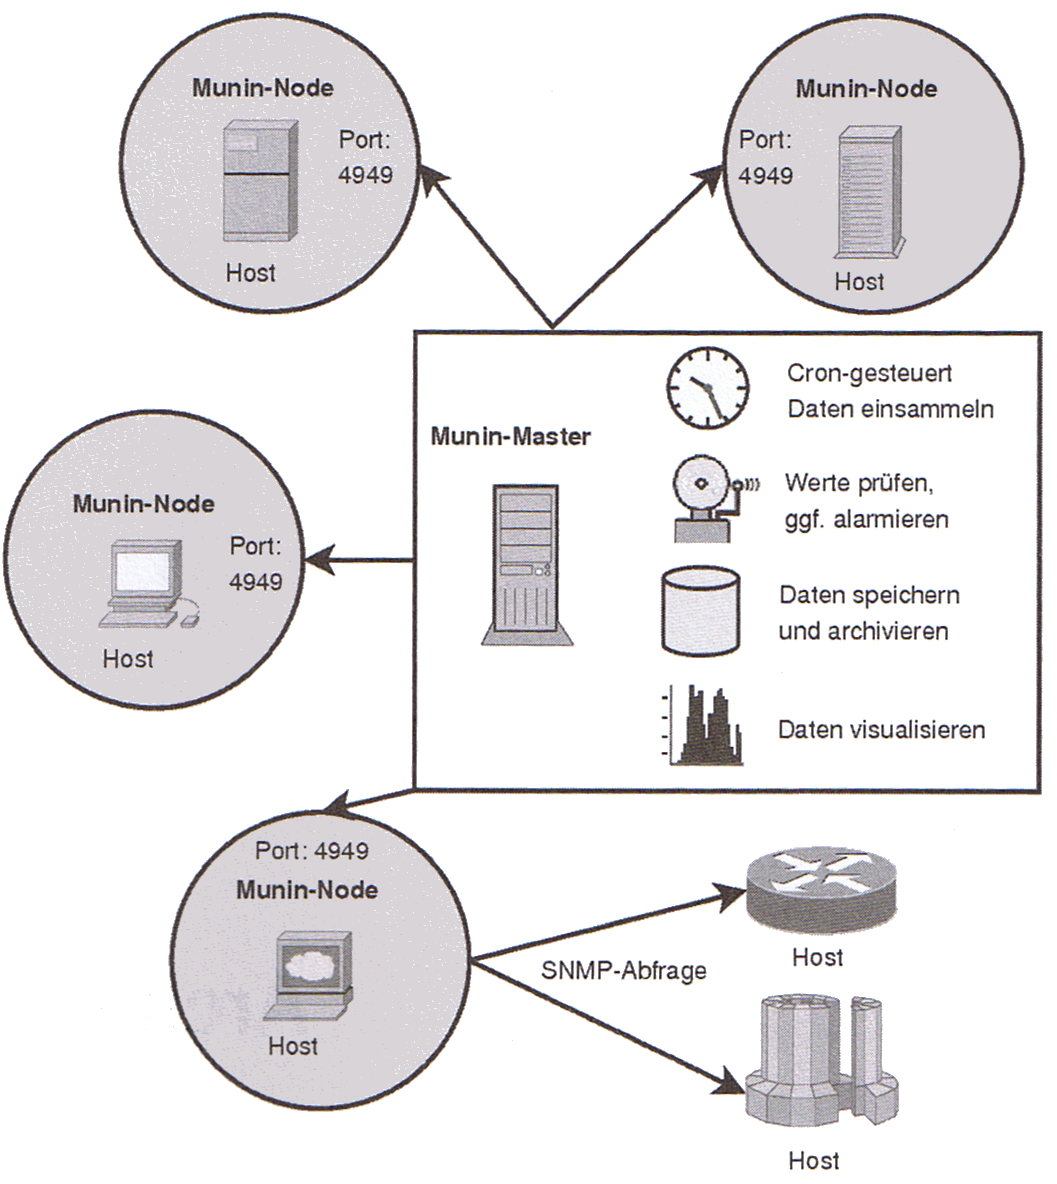
\includegraphics[width=0.85\textwidth]{bilder/master.png}}
		\caption[Munin Master-Node-Konzept]{Munin Master-Node-Konzept\protect\footnotemark}
		\label{master-munin}
\end{figure}
\footnotetext{Quelle: \cite{Mu08} S. 20}

Der Munin-Master ist kein Daemon, sondern besteht aus Skripten, die in regelmäßigen Zeitabstanden als Cron-Job ablaufen:
\begin{itemize}
\item \pictext{munin-update} dient zum Abrufen der Messwerte bei den zu überwachenden Munin-Nodes. Hierbei wird auch die Datenbank aktualisiert oder ggf. erzeugt.
\item \pictext{munin-limits} vergleicht die Messwerte mit ggf. vorgegebenen Schwellwerten und versendet bei Bedarf Benachrichtigungen, wenn Werte das Warnlevel überschreiten, in kritische Bereich gelangen oder wenn Entwarnung gegeben werden kann.
\item \pictext{munin-graph} erzeugt die Munin-Graphen.
\item \pictext{munin-html} dient zum Erstellen der HTML-Seiten der Munin-Übersicht.
\end{itemize}

Standardmäßig werden diese Skripte im fünf Minuten Rythmus aufgerufen.
Dabei baut der Munin-Master viele parallele - im Ausgangszustand unverschlüsselte - TCP-Verbindungen zu den diversen Node-Hosts auf.

Zusätzlich wird für den Betrieb des Munin-Masters auf einem Rechner folgende vorab konfigurierte Software vorausgesetzt:

\begin{itemize}
\item einen Webserver, der Zugang zu den Graphen verschafft.
\item ein Programm mit dem sich die Warnmeldungen versenden lassen. Beispielsweise einen SMTP-Server oder einen Nagios Service Check Acceptor (NSCA), der dafür sorgt, dass der Nagios-Server Alarm schlägt.
\item Werkzeuge und Bibliotheken des \textit{RRDtool}-Projekts\footnote{http://oss.oetiker.ch/rrdtool/} zur Speicherung der Daten und zum Zeichnen der Munin-Graphen.
\end{itemize}


\subsection{Einsammeln der Daten}
Das periodisch ausgeführte Perlskript \pictext{munin-update} kümmert sich um das Abholen neuer Messwerte von den Nodes.
Dazu wird als Erstes die Datei \pictext{munin.conf} geparst, um die zu überwachenden Nodes zu ermitteln.

Ein Eintrag für einen Node-Host in dieser Datei sieht folgendermaßen aus:


\begin{lstlisting}[captionpos=b, caption=Beispielhafte Definition eines Munin-Nodes, label=nodedef, breaklines = true, language=bash]
[munin.example.net]
	address 			localhost
	port				6088
	df.warning			20
	df.critical			10
	contacts			paul
	ping_unilabad.contacts		lang
\end{lstlisting}

Der String in den eckigen Klammern wird als Identifikationsnamen für den Host verwendet und dieser Node wird auch im Webinterface unter diesem Namen aufgelistet.

Das Attribut \textit{address} gibt die IP-Adresse des zu überwachenden Hosts an und mit \textit{port} kann ein vom Standardport (4949) abweichender Port angegeben werden.

Die einzelnen Schwellwerte der verschiedenen Plugins werden auch in diesem Eintrag angegeben, wenn sie von den vorkonfigurierten Werten abweichen sollen.
Dafür wird der Name des Plugins mit den Suffixen \textit{.warning} und \textit{.critical} für die jeweiligen Schwellwerte gesetzt.
Im obigen Beispiel wird \pictext{df} für den freien Festplattenspeicherplatz mit dem Schwellwert von 20\% für Warnungen und 10\% als kritischen Wert für den Host definiert.

Unter dem Attribut \textit{contacts} werden die Kontaktnamen angegeben, die bei einer Überschreitung eines Schwellwerteres kontaktiert werden sollen.
Hierbei gibt es zu sagen, dass diese Überschreitung bei egal welchem Plugin für die Benachrichtigung dieser Kontakte führt.

Soll ein Kontakt nur bei einem bestimmten Plugin benachrichtigt werden, muss es analog zu der Schwellwertdefinition mit dem Pluginnamen und dem Suffix \textit{.contacts} explizit angegeben werden. Hier wird der Kontakt \textit{lang} nur bei einer Überschreitung des Plugins \textit{ping\_unilabad} benachrichtigt.
Bei diesem Plugin wird der Host \textit{unilabad} mit einem Ping überwacht.
Für weitere Details zu dieser Art von Plugin siehe Kapitel \ref{wildcard}.

Weiterhin lässt sich einstellen, dass ein Kontakt generell nur bei kritischen Werten benachrichtigt werden soll.
Die Kontakte müssen zuvor in der \\ \pictext{munin.conf} definiert werden.

Nach der Ermittlung der Nodes werden die Hosts in der Regel parallel nach den neuen Messwerten abgefragt.
Hierfür erzeugt Munin  für jeden in der Konfigurationsdatei angegebenen Rechnern einen eigenen Prozess.
Das parallele Abarbeiten hat den Vorteil, dass die Abfrage nicht bis zum Timeout hängen bleibt, wenn ein einzelner Munin-Node nicht erreichbar ist.
Jedoch verschlingt das Erzeugen eines eigenen Prozesses für jeden Node bei vielen zu überwachenden Rechnern viele Ressourcen, so dass bei größeren Umgebungen viel Arbeitsspeicher und schnelle Multicoreprozessoren unabdingbar sind.

Ein beispielhafte Ausführung eines Munin-Plugins für die Plattenbelegung gibt folgende Werte zurück:

\begin{figure}[ht]
	\centering
	   \fbox{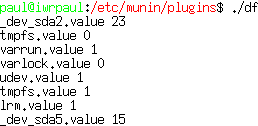
\includegraphics[width=0.6\textwidth]{bilder/df-munin.png}}
		\caption{Beispielhafte Ausführung eines Munin-Plugins}
		\label{df-munin}
\end{figure}
\newpage
Wenn man diese Werte mit den realen Werten vergleicht, erkennt man, dass das Munin-Plugin einfach die Prozentwerte des verbrauchten Speicherplatzes als Wert verwendet.

\begin{figure}[ht]
	\centering
	   \fbox{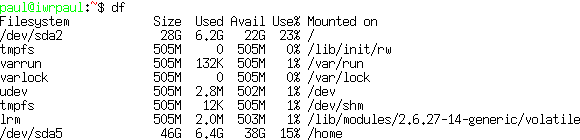
\includegraphics[width=0.85\textwidth]{bilder/df.png}}
		\caption{Reale Werte des Systemtools \textit{df}}
		\label{df}
\end{figure}

Aus diesen Werten erstellt \pictext{munin-graph} automatisch folgenden Graphen:

\begin{figure}[ht]
	\centering
	   \fbox{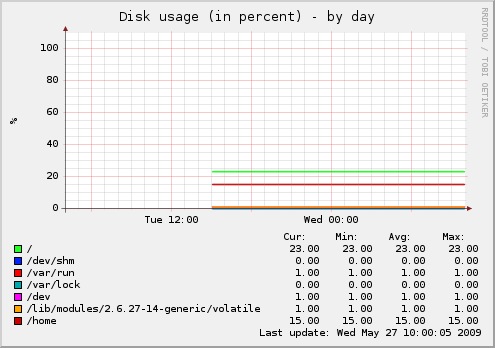
\includegraphics[width=0.85\textwidth]{bilder/df-graph.png}}
		\caption{Visualisierung der Werte des Munin-Plugins \textit{df}}
		\label{df-graph}
\end{figure}

Die über das Netzwerk ermittelten Werte landen nach entsprechender Bearbeitung in RRD-Dateien. 
Im Skript \pictext{munin-update} ist fest eingetragen, welche zeitliche Auflösung die Datenbasis und dadurch auch die Munin-Graphen aufweisen.

Das bedeutet, dass für einen Messpunkt in der Wochenübersicht 30 Minuten - also sechs Messwerte - benötigt werden und für die Monatübersicht werden bereits 48 Messpunkte bzw. zwei Stunden benötigt. Siehe hierfür Tabelle \ref{timeres-tab}.

\begin{table}[!htbp]
\centering
%\begin{twoparttable}
\begin{tabular}{l l}
%\hline
\textbf{Alter der Daten } \hspace{10 mm} & \textbf{Auflösung} \hspace{10 mm} \\
\hline
%\textit{features} & complete\tnote{1} & complete\tnote{1} \\
%\hline
bis zu 30 Stunden & 5 Minuten  \\
\hline
bis zu 9 Tagen & 30 Minuten \\
\hline
bis zu 45 Tagen & 2 Stunden \\
\hline
bis zu 450 Tagen & 1 Tag \\
%\hline
\bottomrule
\end{tabular}
\caption[Zeitliche Auflösung der Datenbasis]{Zeitliche Auflösung der Datenbasis\protect\footnotemark}
\label{timeres-tab}
%\end{twoparttable}
\end{table}
\footnotetext{Quelle: \cite{Mu08} S. 24}


In der Abbildung \ref{4times} konnte der \pictext{munin-node} noch keinen kompletten Tag Messwerte sammeln, weshalb die Jahresübersicht noch keine Messwerte liefern kann und nur mit dem Platzhalterwert \textit{nan} (für nicht defniert) aufgefüllt ist.

\begin{figure}[ht]
	\centering
	   \fbox{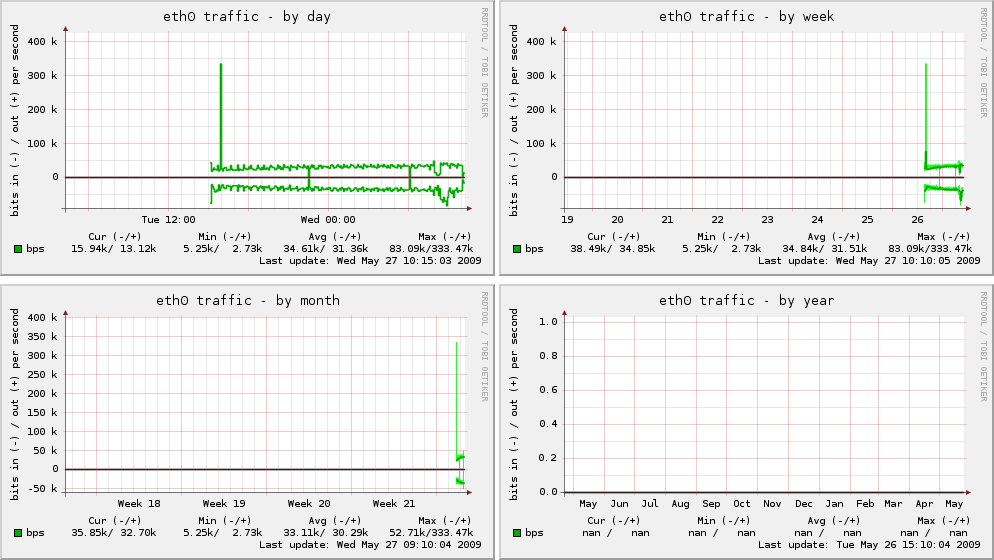
\includegraphics[width=0.9\textwidth]{bilder/4times.png}}
		\caption{Visualisierung der Messwerte in verschiedenen Zeitauflösungen}
		\label{4times}
\end{figure}



\subsection{Round-Robin-Datenbanken}
Round-Robin-Datenbanken sind nicht mit bekannten Datenbanksystemen vergleichbar, da sie in einem proprietären, binären Dateiformat vorliegen.
Daher scheidet der Zugriff per SQL, Texteditor oder über einen Netzwerkport aus.
Um auf Round-Robin-Datenbanken zuzugreifen müssen die dafür entwickelten RRD-Tools verwendet werden.
Diese nehmen die aktuellen Messwerte entgegen und schreiben für jeden Messinterval einen Wert in eine Binärdatei.
Aus dem gesammeltem Datenbestand können dann die Werte visualisiert oder Statistiken erzeugt werden.
Dieser Datenbestand besteht aus sogenannten Round-Robin-Archives.
Dabei handelt es sich um Ableitungen aus den Primärdateien, die mit Hilfe statistischer Auswertungen ermittelt und für die festgelegten Zeitintervalle komprimiert werden.
Die gesamte Anzahl der gespeicherten Datenwerte steht bereits bei der Erzeugung der RRD fest.
Da auch zu Beginn alle Werte mit Platzhaltern aufgefüllt werden, bleibt die Größe einer RRD über die Zeit gleich, siehe Abbildung \ref{rrd-munin}.

\begin{figure}[ht]
	\centering
	   \fbox{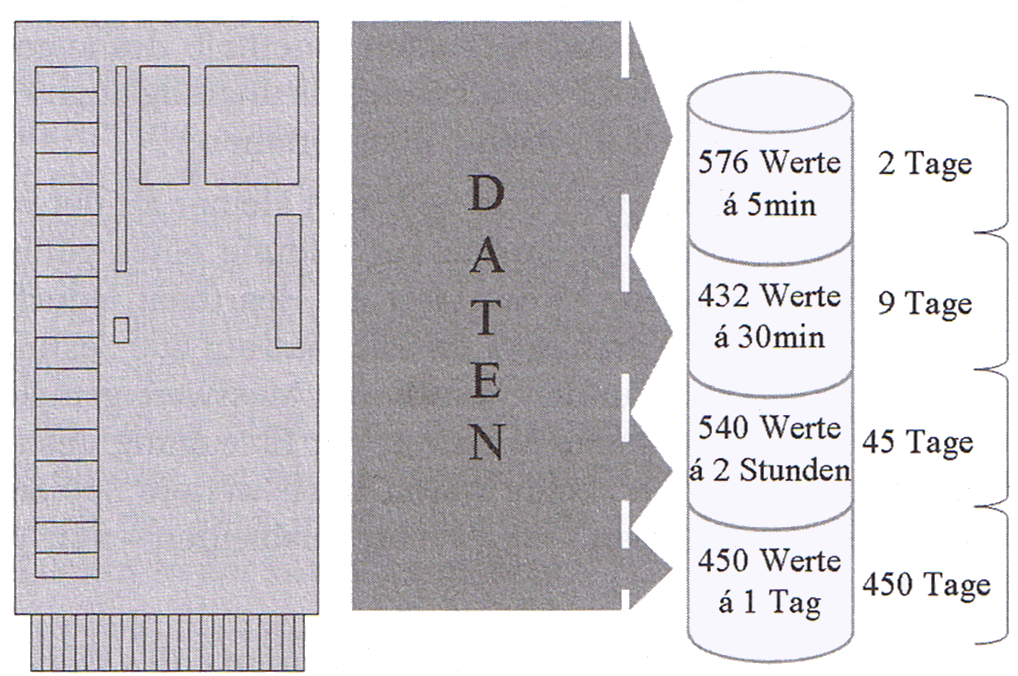
\includegraphics[width=0.76\textwidth]{bilder/rrd.png}}
		\caption[Modell der Round-Robin-Datenbanken]{Modell der Round-Robin-Datenbanken\protect\footnotemark}
		\label{rrd-munin}
\end{figure}
\footnotetext{Quelle: \cite{Mu08} S. 38}

Munin verwendet dieses RRAs als hochauflösende Archive, die die Messwerte des aktuellen Tages, eine etwas komprimierte Fassung zur Darstellung der Daten der laufenden Woche sowie - noch stärker komprimiert - die Daten für den aktuellen Monat und das Jahr enthalten.
%Siehe hierfür Abbildung [?].
Die Komprimierung wird so realisiert, dass Mittelwerte aus der feineren Zeitauflösung errechnet werden und zusätzlich noch spezielle Archivierungsregeln beim Erstellen der RRD-Datei berücksichtigt werden.

Aus diesen Datensätzen mit unterschiedlichen Zeitauflösungen erstellt Munin automatisch Graphen über die entsprechenden Zeiträume, siehe Abbildung \ref{all4}.

\begin{figure}[ht]
	\centering
	   \fbox{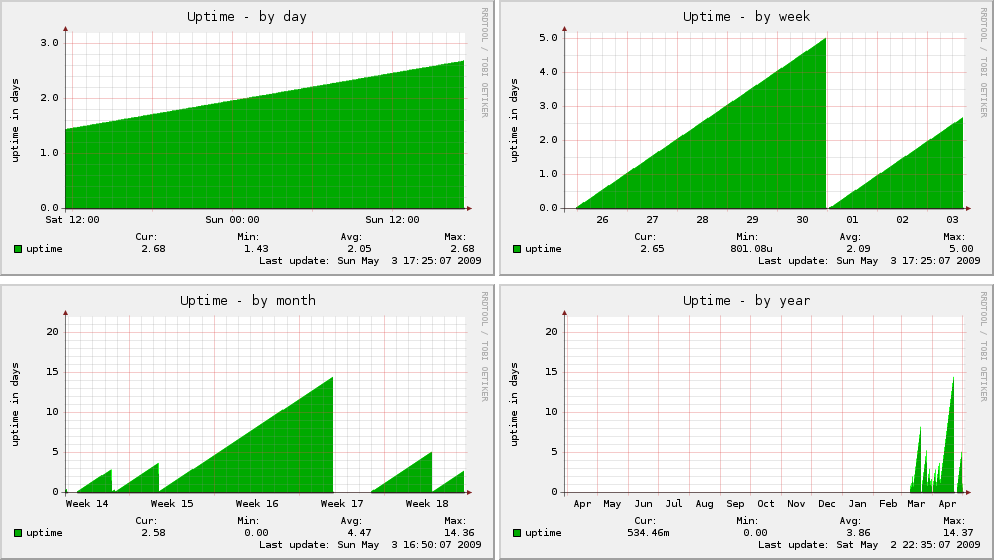
\includegraphics[width=0.95\textwidth]{bilder/all4.png}}
		\caption{Übersicht der \textit{Uptime}}
		\label{all4}
\end{figure}

\newpage

\subsection{Einbindung und Konfiguration der Plugins}
\label{plugins}
Munin bringt bereits eine Sammlung von Plugins bei der Installation mit.
Diese befinden sich in einem Bibliotheksverzeichnis.
Wenn diese Plugins verwendet werden sollen um einen Node zu überwachen, müssen sie in einem Service-Verzeichnis verlinkt sein, damit der Daemon \pictext{munin-node} darauf zugreifen kann.
Dieser Daemon muss sich auf dem zu überwachenden Host befinden und dient als "`Agent"' für den Munin-Master, da der Daemon auf seinem Port nach Aufforderungen durch den Master horcht.
Ein solcher Daemon ist für Linux und für Windows verfügbar, wobei der für Windows weniger Funktionen bietet.
Die einzelnen Tests laufen auf den Nodes unabhängig von der Abfrage des Masters.
Wenn der Master die aktuellen Daten nicht abholt, wird dieser Datenbestand durch die neuen Informationen ausgetauscht und werden bei der nächsten Anfrage an den Master gesendet.

Auf den Graphen im Webinterface wird dieser Zeitraum als Lücke dargestellt, siehe Abbildung \ref{gap}.

\begin{figure}[ht]
	\centering
	   \fbox{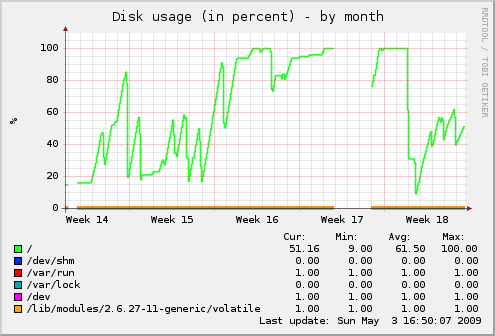
\includegraphics[width=0.852\textwidth]{bilder/gap.png}}
		\caption{Fehlende Messwerte werden als Lücke dargestellt}
		\label{gap}
\end{figure}

Der \pictext{munin-node}-Daemon kannn so konfiguriert werden, dass er nur auf Anfragen von einer bestimmten IP reagiert, einen anderen Port verwendet oder nur auf einer bestimmten IP lauscht.

Damit der Daemon weiss, welche Daten er liefern muss, wird das zuvor erwähnte Service-Verzeichnis verwendet.
Hier werden Verlinkungen zu den eigentlichen Plugins gespeichert.
Eine beispielhafte Verlinkung wird in Abbildung \ref{lns} gezeigt.

\begin{figure}[ht]
	\centering
	   \fbox{
\includegraphics[width=0.85\textwidth]{bilder/lns.png}}
		\caption{Beispielhafte Verlinkung eines Munin-Plugins}
		\label{lns}
\end{figure}

\subsubsection{Wildcard-Plugins}
\label{wildcard}
Falls der Name des Plugins mit einem Unterstrich endet, handelt es sich um ein sogenanntes \textit{Wildcard}-Plugin.
Solche Plugins erwarten in der Bezeichnung des Links spezifische Parameter für die Ausführung der Tests.

Beispielsweise verwendet das zuvor verwendete Plugin \textit{ping\_} als Parameter den Namen oder die IP-Adresse des anzupingenden Hosts.
Die Verlinkung aus dem Bibliotheksverzeichnis in das Service-Verzeichnis würde dann folgendermaßen ausschauen:
\begin{figure}[ht]
	\centering
	   \fbox{
\includegraphics[width=0.85\textwidth]{bilder/lnw.png}}
		\caption{Beispielhafte Verlinkung eines Wildcard-Plugins}
		\label{lnw}
\end{figure}

Hier wird der Host \textit{localhost} angepingt und diese Daten auf dem Master gespeichert und später in einem Graphen visualisiert.

\newpage

\subsubsection{SNMP-Plugins}
Es ist auch möglich Informationen über den zu überwachenden Host in Erfahrung zu bringen, ohne, dass ein \pictext{munin-node}-Daemon auf dem Host installiert ist.
Dies wird durch das Simple Network Management Protocol (SNMP) realisiert.
Durch SNMP kann auf die strukturierte Datenhaltung der MIB in den entfernten Netzwerkknoten zugegriffen werden.
\begin{quote}"`Die Management Information Base (MIB) dient als SNMP-Informations-struktur und besteht aus einem hierarchischen, aus Zahlen aufgebauten Namensraum. Ähnliche Struktur wie andere hierarchische Verzeichnisdiensten wie DNS oder LDAP."'\end{quote}
\begin{flushright}
Quelle: \cite{Barth08} S.233
\end{flushright}

Die MIB-Struktur ist folgendermaßen aufgebaut:

\begin{figure}[ht]
	\centering
	   \fbox{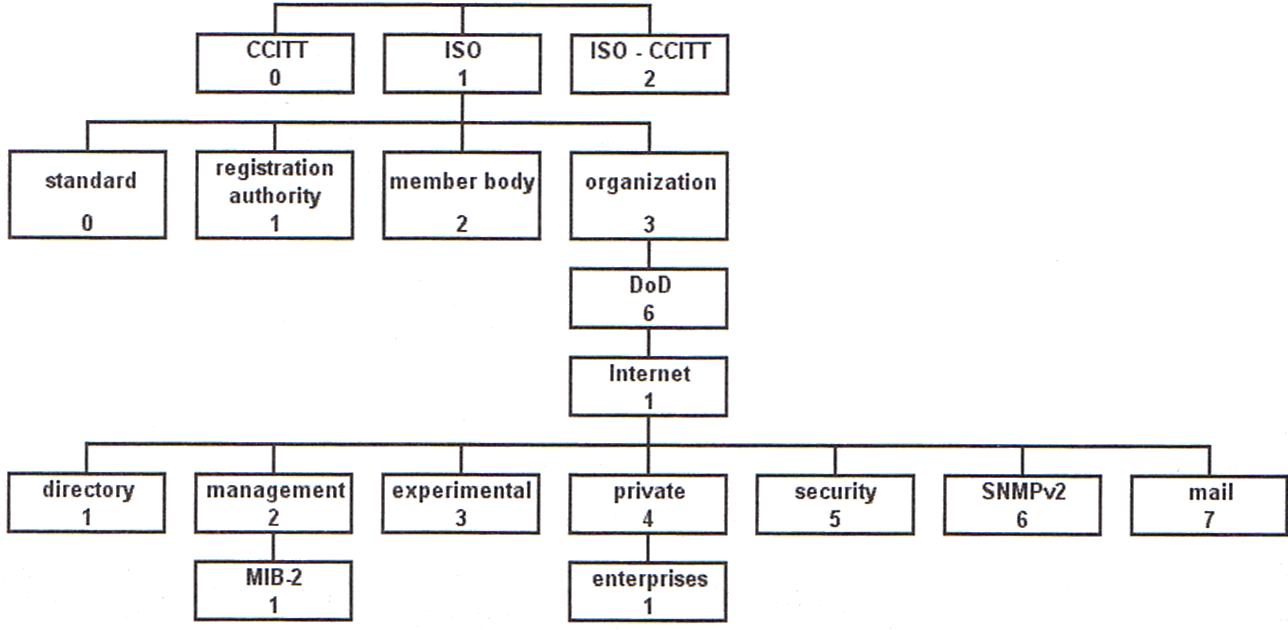
\includegraphics[width=0.95\textwidth]{bilder/mib.png}}
		\caption[Struktur der Management Information Base (MIB)]{Struktur der Management Information Base (MIB)\protect\footnotemark}
		\label{munin-mib}
\end{figure}
\footnotetext{Quelle: \cite{Mu08} S. 156}
Dadurch können die SNMP-Plugins den gewünschten Wert über das Netzwerk abfragen, ohne, dass ein lokal auf dem Munin-Node installiertes Programm notwendig ist.

\newpage

Einen beispielhaften Zugriff auf SNMP-fähige Geräte wird in Abbildung \ref{munin-snmp} gezeigt.

\begin{figure}[ht]
	\centering
	   \fbox{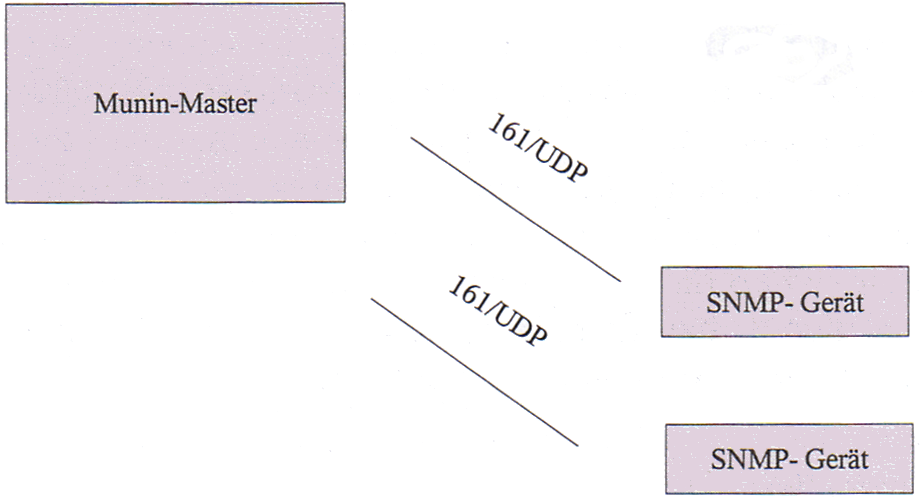
\includegraphics[width=0.85\textwidth]{bilder/snmp.png}}
		\caption[Beispielhafter Zugriff auf SNMP-fähige Geräte]{Beispielhafter Zugriff auf SNMP-fähige Geräte\protect\footnotemark}
		\label{munin-snmp}
\end{figure}
\footnotetext{Quelle: \cite{Mu08} S. 156}

Munin verwendet für SNMP-Plugins eine besondere Namenskonvention.
Alle Plugins dieser Art besitzen den Präfix \textit{snmp\_} auf den die IP-Adresse des SNMP-fähigen Gerätes folgt.
Im folgenden Beispiel wird die Plattenbelegung eines entfernten Knotens überwacht.

\begin{figure}[ht]
	\centering
	   \fbox{
\includegraphics[width=0.85\textwidth]{bilder/snmp-simple.png}}
		\caption{Beispielhafte Verlinkung eines SNMP-Plugins}
		\label{snmp-simple}
\end{figure}

Auch bei diesen SNMP-Plugins gibt es Wildcard-Plugins.
Dabei wird als Suffix im unteren Beispiel der zweite Netzwerkport eines SNMP-fähigen Switches nach Paketfehler abgefragt.

\begin{figure}[ht]
	\centering
	   \fbox{
\includegraphics[width=0.85\textwidth]{bilder/snmp-complex.png}}
		\caption{Beispielhafte Verlinkung eines Wildcard-SNMP-Plugins}
		\label{snmp-complex}
\end{figure}

\newpage

Munin liefert unter anderem folgende SNMP-Plugins mit:

\begin{itemize}
\item \textit{snmp\_\_df} überwacht die Plattenbelegung.
\item \textit{snmp\_\_if\_} ermittelt den Netzwerkdurchsatz.
\item \textit{snmp\_\_if\_err\_} zählt die Paketfehler im Netzwerk.
\item \textit{snmp\_\_sensors\_\_fan} ermittelt die Lüfterdrehzahl.
\item \textit{snmp\_\_load} überwacht die Systemlast.
\item \textit{snmp\_\_processes} ermittelt die Anzahl der laufenden Prozesse.
\item \textit{snmp\_\_users} ermittelt die Anzahl der eingeloggten Benutzer.
\end{itemize}













 \newpage
\section{Umsetzung}
\label{umsetzung}
%Wenn die verwendete Linux-Distributon einen Paketmanager unterstützt 
Unterstützt die verwendete Linux-Distribution einen Paketmanager verläuft die Installation der Anwendung einfach und ohne Probleme.
%Die Installation der Anwendung verläuft einfach und ohne Probleme.
Die hier als Testserver eingesetzte Ubuntu-Distribution verknüpft automatisch die Munin-Webseiten mit dem Webserver und verlinkt bereits die ersten verwendbaren Munin-Plugins.
Aus diesem Grund sind sofort nach der Installation einige Graphen verfügbar, siehe Abbildung \ref{ootb}.

\begin{figure}[ht]
	\centering
	   \fbox{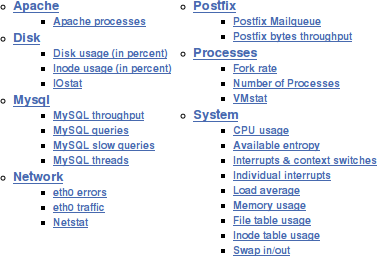
\includegraphics[width=0.8\textwidth]{bilder/ootb.png}}
		\caption{Bereits nach der Installation verfügbare Munin-Graphen}
		\label{ootb}
\end{figure}

Dabei untersucht Munin das verwendete System während der Installation nach verfügbaren Überwachungssobjekten.
Zum Beispiel wurde in der oberen Abbildung von Munin der Mailserver \textit{postfix} gefunden und automatisch in eine eigene Kategorie in das Webinterface eingepflegt.

Wie bereits in Kapitel \ref{plugins} beschrieben können weitere mitgelieferte Munin-Plugins in das entsprechende Service-Verzeichnis verlinkt und dabei ggf. mit Parametern ausgestatten werden, damit Munin zusätzlich diese Graphen erstellt und deren Werte aktualisiert und abspeichert.

Dabei gibt es noch eine zusätzliche Hilfe durch die Plugins, sofern sie sich an den Munin-Plugin-Standard halten.
Solche Skripte überprüfen selbständig bei ihrer Ausführung unter welcher Bedingung sie nicht genutzt werden können oder mit welchen Parametern sie funktionieren würden.

Diese hilfreiche Unterstützung erhält man durch die Ausführung des folgenden Befehls:

\begin{figure}[ht]
	\centering
	   \fbox{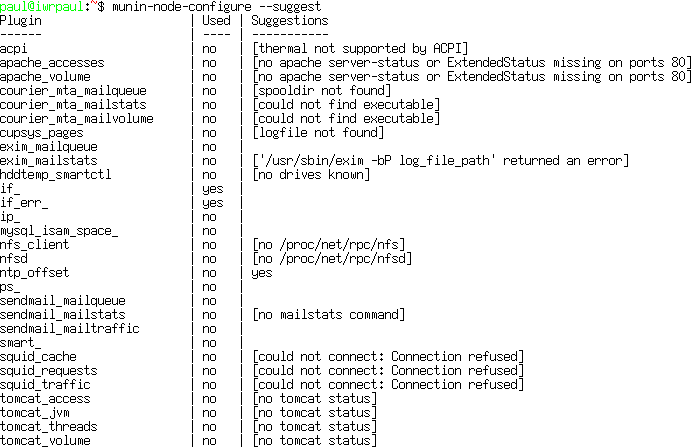
\includegraphics[width=0.9\textwidth]{bilder/suggest.png}}
		\caption{Automatische Überprüfung der Munin-Plugins}
		\label{suggest}
\end{figure}

Anhand dieser Informationen kann herausgefunden werden, weshalb ein Plugin nicht richtig funktioniert oder nicht automatisch bei der Installation hinzugefügt wurde.
\newpage
\subsection{Erstellen eines eigenen Munin-Plugins}

Die zum Zeitpunkt dieser Arbeit mitgelieferten 132 Munin-Plugins unterstützen eine Vielzahl an verschiedenen Überwachungsmöglichkeiten.
Es kann jedoch auch sein, dass ein gewünschtes Element oder Detail nicht von den mitgelieferten Plugins beachtet wird.
Dann bietet es sich an auf der MuninExchange\footnote{http://muninexchange.projects.linpro.no/} Internetseite nach bereits entwickelten, passenden Munin-Plugins zu stöbern.

Eine weitere Möglichkeit besteht darin das gewünschte Skript selbst zu entwickeln.
Da der Aufbau eines Munin-Plugins recht primitiv und klein ausfallen kann, benötigt man keine umfangreichen Programmierkenntnisse um erfolgreich ein funktionierendes Skript zu entwickeln.

Im Folgenden soll als Beispiel eine einfache Speicherplatzüberwachung eines Ordners mit Munin realisiert werden.

Dafür wird das bereits vorhandene Systemtool \textit{du} verwendet.
Der Speicherplatzbedarf eines Ordners lässt sich dann folgendermaßen ermitteln:

\begin{figure}[ht]
	\centering
	   \fbox{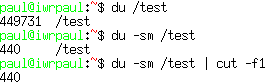
\includegraphics[width=0.55\textwidth]{bilder/du1.png}}
		\caption{Ermittlung des Speicherplatzbedarf des Ordners \textit{/test}}
		\label{du1}
\end{figure}

Mit dem ersten Befehl wird die Verzeichnisgröße des Ordners \textit{/test} gemessen.
Der dabei ermittelte Rückgabewert besitzt KByte als Einheit; da es sich aber um einen etwas größeren Ordner handelt und damit der spätere Munin-Graph nicht zu unübersichtlich wird, bietet es sich an, diese Einheit mit dem zweiten Befehl durch den zusätzlichen Parameter \textit{-sm} in MByte umzurechnen.
Da nur der Speicherplatzbedarf des Ordners interessiert, wird der zweite Teil der Ausgabe mit dem \textit{cut}-Befehl abgeschnitten.

Eine für Munin verwertbare Ausgabe, wie in Abbildung \ref{df-munin}, muss einen internen Variablennamen, in diesem Fall \textit{dir}, gefolgt von dem Suffix \textit{.value}, besitzen.
Daraus ergibt sich folgendes BASH-Skript:

\begin{lstlisting}[captionpos=b, caption=Speicherplatzbedarf eines Verzeichnisses, label=du, breaklines = true, language=bash]
#!/bin/bash
# Plugin to monitor the size of the specified directory
#
# directory to check
DIR="/test"

echo -n "dir.value "
if [ -d $DIR ]; then #check if the dir exists
    SIZE=`du -sm $DIR | cut -f1`
    echo $SIZE
    exit 0
else
    echo "Error: check your directory!"
    exit 1
fi
\end{lstlisting}

Nach der Verlinkung in das entsprechende Service-Verzeichnis gibt das Skriptes folgende Ausgabe zurück:

\begin{figure}[ht]
	\centering
	   \fbox{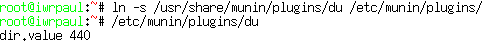
\includegraphics[width=0.85\textwidth]{bilder/du2.png}}
		\caption{Ausführung des Testplugins}
		\label{du2}
\end{figure}

Mit dieser Ausgabe kann \pictext{munin-update} die Messwerte ermitteln und speichern.

Für die Visualisierung dieser Messwerte benötigt Munin zusätzlich noch Informationen, wie der Graph auszusehen hat.
Um diese Informationen zu erhalten, ruft Munin die Plugins mit dem Parameter \textit{config} auf; daher muss auch dieses Plugin die entsprechende Werte bei diesem Parameteraufruf liefern.

Folgende Informationen werden für das Testplugin benötigt:

\begin{itemize}
\item \textit{graph\_title} als Titel für den Graphen
\item \textit{graph\_vlabel} als Beschriftung der y-Achse
\item \textit{graph\_category} für die Kategorie in welche der resultierende Graph eingeordnet werden soll
\item \textit{dir.label} als Bezeichnung der Messwerte
\item \textit{dir.min} als Minimalwert der Messwerte
\item \textit{dir.info} zusätzliche Beschreibung unterhalb des Graphen
\end{itemize}

Der dafür benötigte Quelltext wird vor der eigentlichen Messwertermittlung eingeschoben, da sich das Skript ansonsten zuvor mit \textit{exit} beendet.
Das fertige Skript sieht dann folgendermaßen aus:

\begin{lstlisting}[captionpos=b, caption=Fertiges Skript für den Speicherplatzbedarf eines Verzeichnisses, label=du, breaklines = true, language=bash]
#!/bin/bash
# Plugin to monitor the size of the specified directory
#
# directory to check
DIR="/test"

if [ "$1" = "config" ]; then
	echo "graph_title Directory size: $DIR"
	echo "graph_vlabel size MB"
	echo "graph_category disk"
	echo "graph_info Size of $DIR"
	echo "dir.label size"
	echo "dir.min 0"
	echo "dir.info Shows du -sm for specified directory"
	exit 0
fi

echo -n "dir.value "
if [ -d $DIR ]; then #check if the dir exists
    SIZE=`du -sm $DIR | cut -f1`
    echo $SIZE
    exit 0
else
    echo "Error: check your directory!"
    exit 1
fi
\end{lstlisting}

Nach dem Neustarten des \pictext{munin-node}-Daemons wird folgender Graph im Webinterface angezeigt:

\begin{figure}[ht]
	\centering
	   \fbox{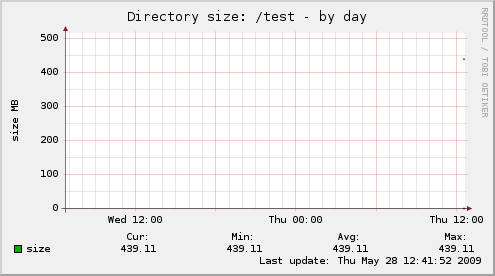
\includegraphics[width=0.85\textwidth]{bilder/du-graph.png}}
		\caption{Fertiger Muningraph des Testskriptes}
		\label{du-graph}
\end{figure}

Dies ist nur ein simples Beispiel für ein eigenes Munin-Plugin.
Dem Entwickler sind aber fast keine Grenzen gesetzt, solange er sich an die von Munin benötigten Werte hält. \newpage
\subsection{Zusammenspiel mit Nagios}

Nagios dient zum Überwachen von Hosts und deren Services in komplexeren Infrastrukturen und bietet viele zusätzliche Features.
Es gibt einige essentielle Unterschiede zwischen den beiden Überwachungsanwendungen.
Während Munin mehr Wert auf die Visualisierung der Überwachungsdaten legt, kümmert sich Nagios intensiver um die Überwachungs- und Alarmierungslogik.
Beispielsweise überwacht Munin ständig die Überschreitung von den angegebenen Schwellwerten und schlägt ggf. Alarm.
Im Gegensatz hierzu wird bei Nagios mit Hard- und Soft-States gearbeitet, bei denen sich der Fehler erst durch mehrmaliges Überprüfen als "`True Positive"' beweisen muss.

Dies ist nur ein Beispiel für die überlegene Überwachungslogik von Nagios, doch Munin wurde nicht in der Absicht entwickelt mit Nagios zu konkurrieren.
Das genaue Gegenteil ist der Fall - Nagios und Munin können zusammenarbeiten.

Es ist durchaus denkbar, dass bereits ein Nagios-Überwachungssytem in der Netzwerkstruktur betrieben wird.
Eine zusätzliche Benachrichtigung von Fehlern bzw. Warnungen und die dezentrale Aufsplittung der Überwachung in zwei getrennte Systeme ist in den meisten Fällen ineffizient und daher nicht gewollt.

Deshalb gibt es die Möglichkeit die vorhandene Nagios-Instanz als "`Event-Handler"' für die von Munin festgestellten Überschreitungen von Schwellwerten zu verwenden.

Dabei wird, anstatt der Alarmierung durch Emails, ein passives Check-Ergebnis mittels \pictext{send\_nsca} an den Nagios Server versendet.
Dieser nimmt das Ergebnis entgegen und benachrichtigt die entsprechenden Benutzer.
Damit Nagios solche passiven Ergebnisse aufnehmen kann, muss sich auf dem Nagios-Server ein NSCA-Daemon (Nagios Service Check Acceptor) befinden, der auf dem entsprechenden Port auf die Benachrichtigungen wartet.

In folgender Abbildung wird ein beispielhafter Aufbau eines solchen Systems gezeigt, welches die Kommunikation zwischen Nagios und Munin verdeutlichen soll:

\begin{figure}[ht]
	\centering
	   \fbox{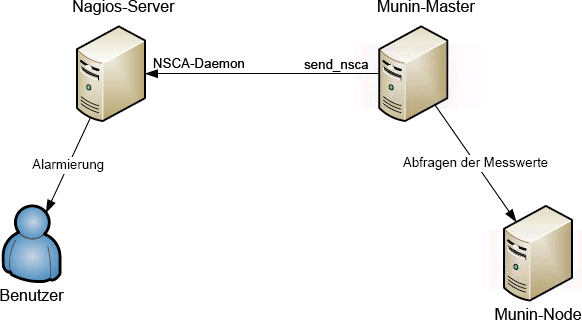
\includegraphics[width=0.9\textwidth]{bilder/nsca.png}}
		\caption{Zusammenarbeit von Munin und Nagios}
		\label{nsca}
\end{figure}

\begin{enumerate}
\item Der Munin-Master sammelt in periodischen Abläufen die Messwerte ab, welche ständig von den Munin-Nodes selbst ermittelt werden.
\item Die Messwerte werden vom Master überprüft.
\item Bei einer Überschreitung wird, anstatt einer Email, das Tool \pictext{send\_nsca} dazu verwendet, den Nagios-Server darüber zu benachrichtigen.
\item Der auf dem Nagios-Server laufende NSCA-Daemon nimmt das Ergebnis des Munin-Masters als passives Check-Ergebnis entgegen und filtert nochmals nach seinen eigenen Benachrichtigungs- und Eskalationsregeln.
\item Bei einer notwendigen Alarmierung nimmt Nagios Kontakt mit den zuständigen Benutzern auf.
\end{enumerate}

\subsection{Vergleich der Visualisierung mit Nagios}

Nagios bietet standardmäßig keine Visualisierung der Überwachungsdaten an.

Durch verschiedene Addons lässt sich dies jedoch nachträglich hinzufügen.

Solche Addons sind zum Beispiel:
\begin{itemize}
\item Nagiosgraph 

\begin{figure}[ht]
	\centering
	   \fbox{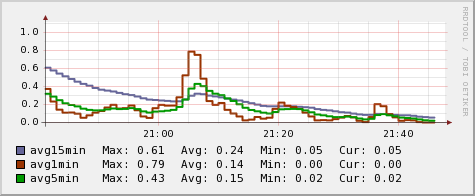
\includegraphics[width=0.9\textwidth]{bilder/nagiosgraph.png}}
		\caption{Visualisierung der Performancedaten mit Nagiosgraph}
		\label{nagiosgraph}
\end{figure}

\item drraw

\begin{figure}[ht]
	\centering
	   \fbox{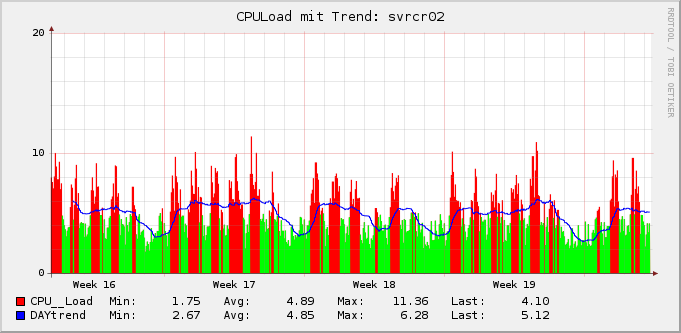
\includegraphics[width=0.85\textwidth]{bilder/drraw.png}}
		\caption{Visualisierung der Performancedaten mit drraw}
		\label{drraw}
\end{figure}

\newpage
\item NagiosGrapher

\begin{figure}[ht]
	\centering
	   \fbox{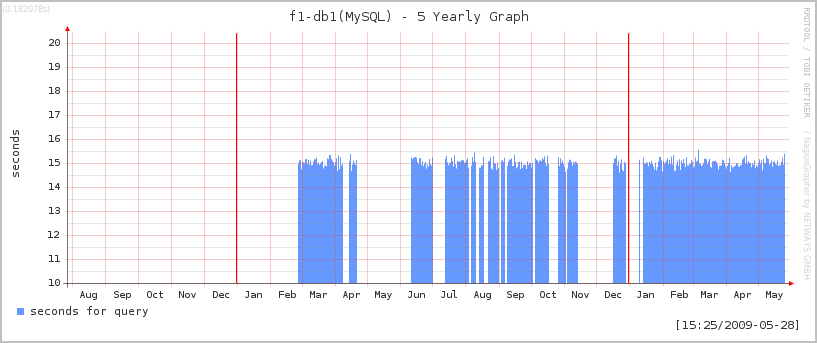
\includegraphics[width=0.9\textwidth]{bilder/nagios.png}}
		\caption{Visualisierung der Performancedaten mit NagiosGrapher}
		\label{nagios}
\end{figure}

\item Perf2rrd

\begin{figure}[ht]
	\centering
	   \fbox{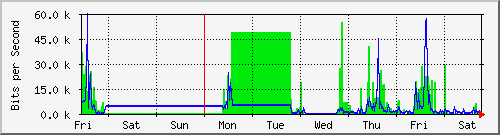
\includegraphics[width=0.85\textwidth]{bilder/perf2rdd.png}}
		\caption{Visualisierung der Performancedaten mit Perf2rrd}
		\label{perf2rdd}
\end{figure}
\end{itemize}

Allgemein lässt sich sagen, dass die Visualisierung der Überwachungsdaten durch Nagios als unerfahrener Benutzer deutlich aufwändiger ist als mit Munin, da alleine die Entscheidung für ein Addon und dessen Konfiguration bis zum ersten Graphen länger als eine vollständige Munin Installation dauert.
Dafür stehen mit den Nagios-Visualisierungs-Addon mehr Möglichkeiten zur Verfügung, indem zum Beispiel die Performanzedaten länger als ein Jahr gespeichert werden können, wie in vorheriger Abbildung \ref{nagios}, mit einem Zeitverlauf über fünf Jahren, gezeigt.

 \newpage
\section{Zusammenfassung und Ausblick}
Die von Munin zusammengetragenen Informationen sind dank der einfachen Installation der Anwendung und der gewünschten Munin-Plugins sehr schnell in nützliche Graphen umgewandelt und erweisen sich dank der verschiedenen Zeitauflösung als sehr nützliches Element in der Langzeitüberwachung.

Auch die große Anzahl an bereits bei der Installation verfügbaren Plugins lassen sich dank einer automatischen Testfunktion, siehe Abbildung \ref{suggest} in Kapitel \ref{umsetzung}, schnell und unkompliziert einbinden.

Sollte sich doch nicht das passende Plugin in dieser Sammlung finden, gibt es immernoch die Möglichkeit auf der MuninExchange Internetseite fündig zu werden.
Dort befinden sich von anderen Munin-Benutzern entwickelte und veröffentlichte Plugins, die auch weiter vom Benutzer auf die eigenen Bedürfnisse angepasst werden können.
Da die Plugins jedoch recht einfach aufgebaut sind, lassen sich auch schnell und einfach eigene Kreationen entwerfen, die sofort automatisch nach der Verlinkung zum Service-Verzeichnis in das Webinterface eingefügt werden.

Munin legt großen Wert auf die Visualisierung der Überwachungsinformationen und weniger auf eine komplexe, umfangreiche Überwachungs- und Alarmierungslogik.
Dafür empfiehlt es sich für diesen Zweck Nagios zu verwenden und Munin in das Nagios Überwachungssytem einzubinden.
Denn sowohl Nagios als auch Munin bieten die notwendigen Werkzeuge um dies zu realisieren.
Dabei muss erwähnt werden, dass auch mit Nagios die Visualisierung der Performancedaten der Plugins möglich ist, so dass Munin als überflüssig gesehn werden könnte.
Jedoch stellt sich die Konfiguration und Anpassung von Nagios und dem Visualisierung-Addon für den unerfahrenen Benutzer als deutlich schwieriger und aufwändiger heraus als der Aufbau eines ähnlichen Munin Überwachungssystems. \newpage
%\section{Architektur}

Munin verwendet eine sogenannte Master-Node-Architektur, siehe Abbildung \ref{master-munin}.
Hierbei emittelt jeder Rechner seine Messwerte selbst und der Master holt sich diese Daten mittels diverser Agenten, den sogenannten Munin-Nodes, ab.
Deshalb wird der Master lediglich zur Verarbeitung der Überwachungsdaten genutzt.

\begin{figure}[ht]
	\centering
	   \fbox{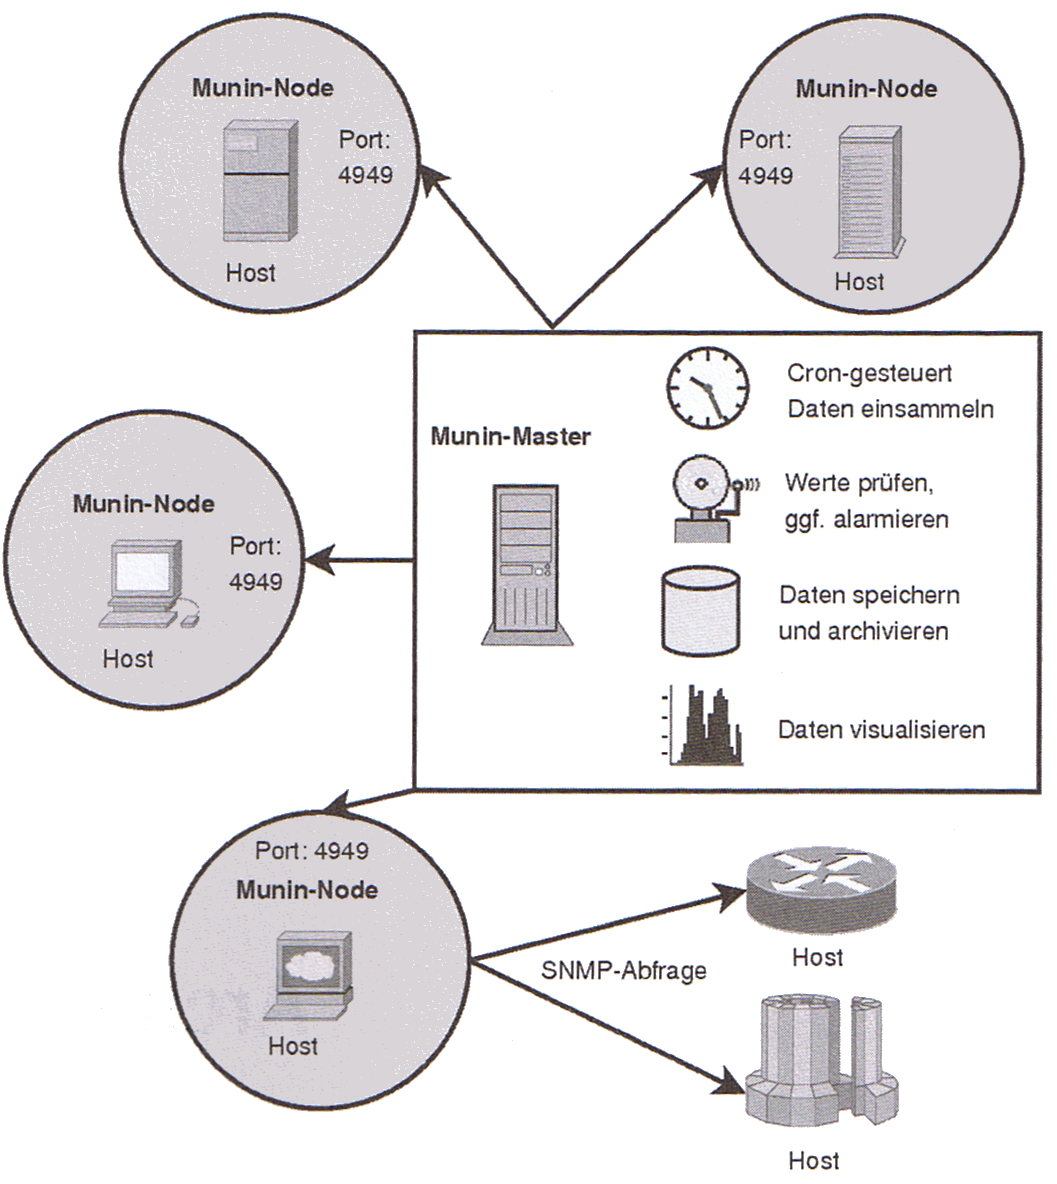
\includegraphics[width=0.85\textwidth]{bilder/master.png}}
		\caption[Munin Master-Node-Konzept]{Munin Master-Node-Konzept\protect\footnotemark}
		\label{master-munin}
\end{figure}
\footnotetext{Quelle: \cite{Mu08} S. 20}

Der Munin-Master ist kein Daemon, sondern besteht aus Skripten, die in regelmäßigen Zeitabstanden als Cron-Job ablaufen:
\begin{itemize}
\item \pictext{munin-update} dient zum Abrufen der Messwerte bei den zu überwachenden Munin-Nodes. Hierbei wird auch die Datenbank aktualisiert oder ggf. erzeugt.
\item \pictext{munin-limits} vergleicht die Messwerte mit ggf. vorgegebenen Schwellwerten und versendet bei Bedarf Benachrichtigungen, wenn Werte das Warnlevel überschreiten, in kritische Bereich gelangen oder wenn Entwarnung gegeben werden kann.
\item \pictext{munin-graph} erzeugt die Munin-Graphen.
\item \pictext{munin-html} dient zum Erstellen der HTML-Seiten der Munin-Übersicht.
\end{itemize}

Standardmäßig werden diese Skripte im fünf Minuten Rythmus aufgerufen.
Dabei baut der Munin-Master viele parallele - im Ausgangszustand unverschlüsselte - TCP-Verbindungen zu den diversen Node-Hosts auf.

Zusätzlich wird für den Betrieb des Munin-Masters auf einem Rechner folgende vorab konfigurierte Software vorausgesetzt:

\begin{itemize}
\item einen Webserver, der Zugang zu den Graphen verschafft.
\item ein Programm mit dem sich die Warnmeldungen versenden lassen. Beispielsweise einen SMTP-Server oder einen Nagios Service Check Acceptor (NSCA), der dafür sorgt, dass der Nagios-Server Alarm schlägt.
\item Werkzeuge und Bibliotheken des \textit{RRDtool}-Projekts\footnote{http://oss.oetiker.ch/rrdtool/} zur Speicherung der Daten und zum Zeichnen der Munin-Graphen.
\end{itemize}


\subsection{Einsammeln der Daten}
Das periodisch ausgeführte Perlskript \pictext{munin-update} kümmert sich um das Abholen neuer Messwerte von den Nodes.
Dazu wird als Erstes die Datei \pictext{munin.conf} geparst, um die zu überwachenden Nodes zu ermitteln.

Ein Eintrag für einen Node-Host in dieser Datei sieht folgendermaßen aus:


\begin{lstlisting}[captionpos=b, caption=Beispielhafte Definition eines Munin-Nodes, label=nodedef, breaklines = true, language=bash]
[munin.example.net]
	address 			localhost
	port				6088
	df.warning			20
	df.critical			10
	contacts			paul
	ping_unilabad.contacts		lang
\end{lstlisting}

Der String in den eckigen Klammern wird als Identifikationsnamen für den Host verwendet und dieser Node wird auch im Webinterface unter diesem Namen aufgelistet.

Das Attribut \textit{address} gibt die IP-Adresse des zu überwachenden Hosts an und mit \textit{port} kann ein vom Standardport (4949) abweichender Port angegeben werden.

Die einzelnen Schwellwerte der verschiedenen Plugins werden auch in diesem Eintrag angegeben, wenn sie von den vorkonfigurierten Werten abweichen sollen.
Dafür wird der Name des Plugins mit den Suffixen \textit{.warning} und \textit{.critical} für die jeweiligen Schwellwerte gesetzt.
Im obigen Beispiel wird \pictext{df} für den freien Festplattenspeicherplatz mit dem Schwellwert von 20\% für Warnungen und 10\% als kritischen Wert für den Host definiert.

Unter dem Attribut \textit{contacts} werden die Kontaktnamen angegeben, die bei einer Überschreitung eines Schwellwerteres kontaktiert werden sollen.
Hierbei gibt es zu sagen, dass diese Überschreitung bei egal welchem Plugin für die Benachrichtigung dieser Kontakte führt.

Soll ein Kontakt nur bei einem bestimmten Plugin benachrichtigt werden, muss es analog zu der Schwellwertdefinition mit dem Pluginnamen und dem Suffix \textit{.contacts} explizit angegeben werden. Hier wird der Kontakt \textit{lang} nur bei einer Überschreitung des Plugins \textit{ping\_unilabad} benachrichtigt.
Bei diesem Plugin wird der Host \textit{unilabad} mit einem Ping überwacht.
Für weitere Details zu dieser Art von Plugin siehe Kapitel \ref{wildcard}.

Weiterhin lässt sich einstellen, dass ein Kontakt generell nur bei kritischen Werten benachrichtigt werden soll.
Die Kontakte müssen zuvor in der \\ \pictext{munin.conf} definiert werden.

Nach der Ermittlung der Nodes werden die Hosts in der Regel parallel nach den neuen Messwerten abgefragt.
Hierfür erzeugt Munin  für jeden in der Konfigurationsdatei angegebenen Rechnern einen eigenen Prozess.
Das parallele Abarbeiten hat den Vorteil, dass die Abfrage nicht bis zum Timeout hängen bleibt, wenn ein einzelner Munin-Node nicht erreichbar ist.
Jedoch verschlingt das Erzeugen eines eigenen Prozesses für jeden Node bei vielen zu überwachenden Rechnern viele Ressourcen, so dass bei größeren Umgebungen viel Arbeitsspeicher und schnelle Multicoreprozessoren unabdingbar sind.

Ein beispielhafte Ausführung eines Munin-Plugins für die Plattenbelegung gibt folgende Werte zurück:

\begin{figure}[ht]
	\centering
	   \fbox{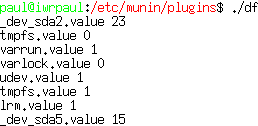
\includegraphics[width=0.6\textwidth]{bilder/df-munin.png}}
		\caption{Beispielhafte Ausführung eines Munin-Plugins}
		\label{df-munin}
\end{figure}
\newpage
Wenn man diese Werte mit den realen Werten vergleicht, erkennt man, dass das Munin-Plugin einfach die Prozentwerte des verbrauchten Speicherplatzes als Wert verwendet.

\begin{figure}[ht]
	\centering
	   \fbox{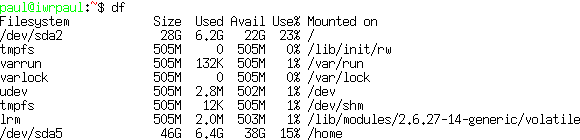
\includegraphics[width=0.85\textwidth]{bilder/df.png}}
		\caption{Reale Werte des Systemtools \textit{df}}
		\label{df}
\end{figure}

Aus diesen Werten erstellt \pictext{munin-graph} automatisch folgenden Graphen:

\begin{figure}[ht]
	\centering
	   \fbox{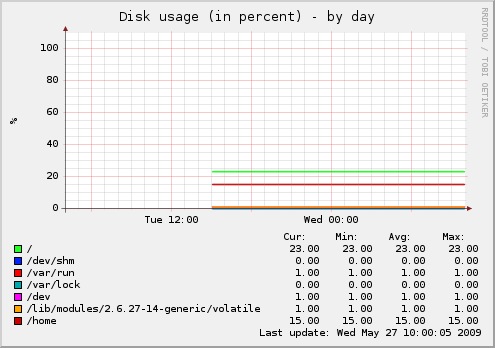
\includegraphics[width=0.85\textwidth]{bilder/df-graph.png}}
		\caption{Visualisierung der Werte des Munin-Plugins \textit{df}}
		\label{df-graph}
\end{figure}

Die über das Netzwerk ermittelten Werte landen nach entsprechender Bearbeitung in RRD-Dateien. 
Im Skript \pictext{munin-update} ist fest eingetragen, welche zeitliche Auflösung die Datenbasis und dadurch auch die Munin-Graphen aufweisen.

Das bedeutet, dass für einen Messpunkt in der Wochenübersicht 30 Minuten - also sechs Messwerte - benötigt werden und für die Monatübersicht werden bereits 48 Messpunkte bzw. zwei Stunden benötigt. Siehe hierfür Tabelle \ref{timeres-tab}.

\begin{table}[!htbp]
\centering
%\begin{twoparttable}
\begin{tabular}{l l}
%\hline
\textbf{Alter der Daten } \hspace{10 mm} & \textbf{Auflösung} \hspace{10 mm} \\
\hline
%\textit{features} & complete\tnote{1} & complete\tnote{1} \\
%\hline
bis zu 30 Stunden & 5 Minuten  \\
\hline
bis zu 9 Tagen & 30 Minuten \\
\hline
bis zu 45 Tagen & 2 Stunden \\
\hline
bis zu 450 Tagen & 1 Tag \\
%\hline
\bottomrule
\end{tabular}
\caption[Zeitliche Auflösung der Datenbasis]{Zeitliche Auflösung der Datenbasis\protect\footnotemark}
\label{timeres-tab}
%\end{twoparttable}
\end{table}
\footnotetext{Quelle: \cite{Mu08} S. 24}


In der Abbildung \ref{4times} konnte der \pictext{munin-node} noch keinen kompletten Tag Messwerte sammeln, weshalb die Jahresübersicht noch keine Messwerte liefern kann und nur mit dem Platzhalterwert \textit{nan} (für nicht defniert) aufgefüllt ist.

\begin{figure}[ht]
	\centering
	   \fbox{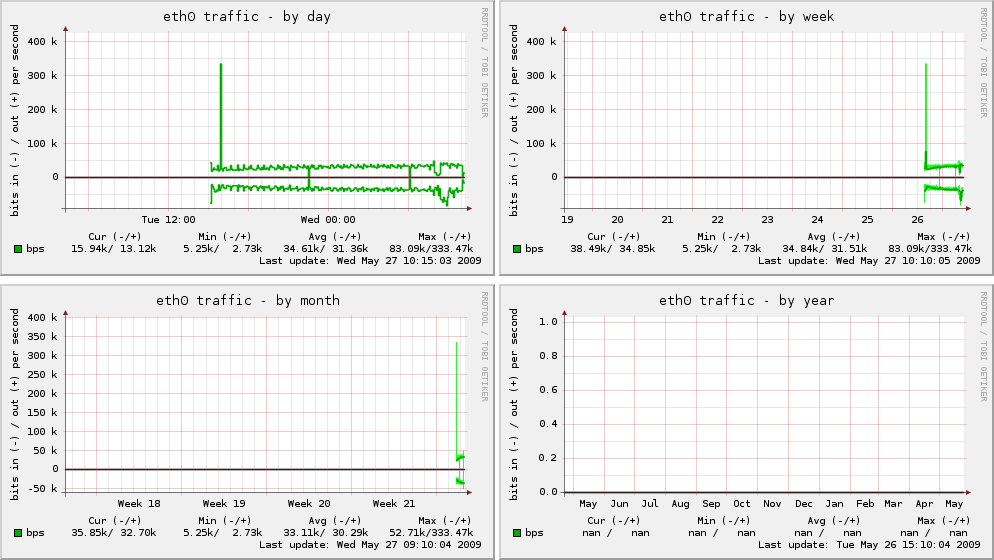
\includegraphics[width=0.9\textwidth]{bilder/4times.png}}
		\caption{Visualisierung der Messwerte in verschiedenen Zeitauflösungen}
		\label{4times}
\end{figure}



\subsection{Round-Robin-Datenbanken}
Round-Robin-Datenbanken sind nicht mit bekannten Datenbanksystemen vergleichbar, da sie in einem proprietären, binären Dateiformat vorliegen.
Daher scheidet der Zugriff per SQL, Texteditor oder über einen Netzwerkport aus.
Um auf Round-Robin-Datenbanken zuzugreifen müssen die dafür entwickelten RRD-Tools verwendet werden.
Diese nehmen die aktuellen Messwerte entgegen und schreiben für jeden Messinterval einen Wert in eine Binärdatei.
Aus dem gesammeltem Datenbestand können dann die Werte visualisiert oder Statistiken erzeugt werden.
Dieser Datenbestand besteht aus sogenannten Round-Robin-Archives.
Dabei handelt es sich um Ableitungen aus den Primärdateien, die mit Hilfe statistischer Auswertungen ermittelt und für die festgelegten Zeitintervalle komprimiert werden.
Die gesamte Anzahl der gespeicherten Datenwerte steht bereits bei der Erzeugung der RRD fest.
Da auch zu Beginn alle Werte mit Platzhaltern aufgefüllt werden, bleibt die Größe einer RRD über die Zeit gleich, siehe Abbildung \ref{rrd-munin}.

\begin{figure}[ht]
	\centering
	   \fbox{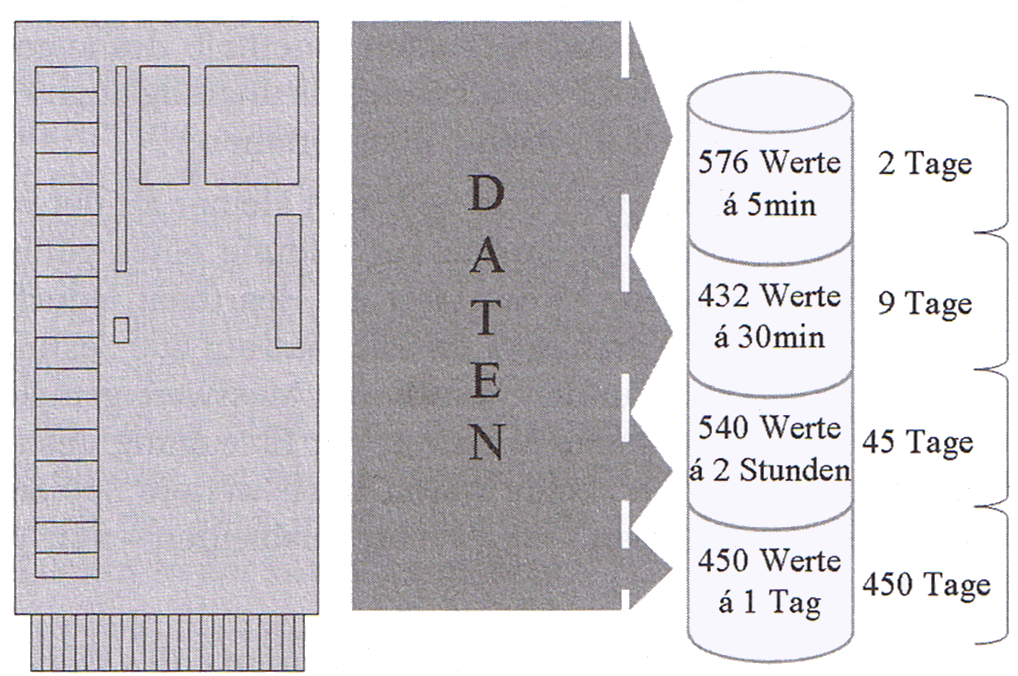
\includegraphics[width=0.76\textwidth]{bilder/rrd.png}}
		\caption[Modell der Round-Robin-Datenbanken]{Modell der Round-Robin-Datenbanken\protect\footnotemark}
		\label{rrd-munin}
\end{figure}
\footnotetext{Quelle: \cite{Mu08} S. 38}

Munin verwendet dieses RRAs als hochauflösende Archive, die die Messwerte des aktuellen Tages, eine etwas komprimierte Fassung zur Darstellung der Daten der laufenden Woche sowie - noch stärker komprimiert - die Daten für den aktuellen Monat und das Jahr enthalten.
%Siehe hierfür Abbildung [?].
Die Komprimierung wird so realisiert, dass Mittelwerte aus der feineren Zeitauflösung errechnet werden und zusätzlich noch spezielle Archivierungsregeln beim Erstellen der RRD-Datei berücksichtigt werden.

Aus diesen Datensätzen mit unterschiedlichen Zeitauflösungen erstellt Munin automatisch Graphen über die entsprechenden Zeiträume, siehe Abbildung \ref{all4}.

\begin{figure}[ht]
	\centering
	   \fbox{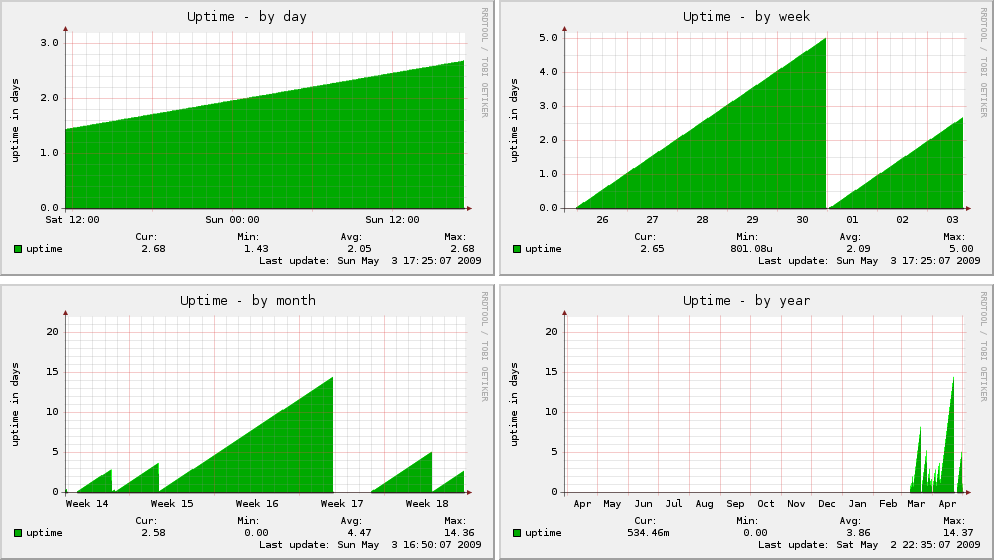
\includegraphics[width=0.95\textwidth]{bilder/all4.png}}
		\caption{Übersicht der \textit{Uptime}}
		\label{all4}
\end{figure}

\newpage

\subsection{Einbindung und Konfiguration der Plugins}
\label{plugins}
Munin bringt bereits eine Sammlung von Plugins bei der Installation mit.
Diese befinden sich in einem Bibliotheksverzeichnis.
Wenn diese Plugins verwendet werden sollen um einen Node zu überwachen, müssen sie in einem Service-Verzeichnis verlinkt sein, damit der Daemon \pictext{munin-node} darauf zugreifen kann.
Dieser Daemon muss sich auf dem zu überwachenden Host befinden und dient als "`Agent"' für den Munin-Master, da der Daemon auf seinem Port nach Aufforderungen durch den Master horcht.
Ein solcher Daemon ist für Linux und für Windows verfügbar, wobei der für Windows weniger Funktionen bietet.
Die einzelnen Tests laufen auf den Nodes unabhängig von der Abfrage des Masters.
Wenn der Master die aktuellen Daten nicht abholt, wird dieser Datenbestand durch die neuen Informationen ausgetauscht und werden bei der nächsten Anfrage an den Master gesendet.

Auf den Graphen im Webinterface wird dieser Zeitraum als Lücke dargestellt, siehe Abbildung \ref{gap}.

\begin{figure}[ht]
	\centering
	   \fbox{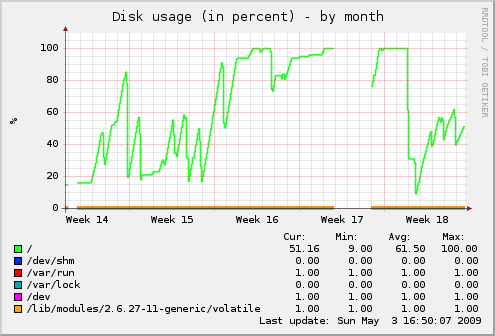
\includegraphics[width=0.852\textwidth]{bilder/gap.png}}
		\caption{Fehlende Messwerte werden als Lücke dargestellt}
		\label{gap}
\end{figure}

Der \pictext{munin-node}-Daemon kannn so konfiguriert werden, dass er nur auf Anfragen von einer bestimmten IP reagiert, einen anderen Port verwendet oder nur auf einer bestimmten IP lauscht.

Damit der Daemon weiss, welche Daten er liefern muss, wird das zuvor erwähnte Service-Verzeichnis verwendet.
Hier werden Verlinkungen zu den eigentlichen Plugins gespeichert.
Eine beispielhafte Verlinkung wird in Abbildung \ref{lns} gezeigt.

\begin{figure}[ht]
	\centering
	   \fbox{
\includegraphics[width=0.85\textwidth]{bilder/lns.png}}
		\caption{Beispielhafte Verlinkung eines Munin-Plugins}
		\label{lns}
\end{figure}

\subsubsection{Wildcard-Plugins}
\label{wildcard}
Falls der Name des Plugins mit einem Unterstrich endet, handelt es sich um ein sogenanntes \textit{Wildcard}-Plugin.
Solche Plugins erwarten in der Bezeichnung des Links spezifische Parameter für die Ausführung der Tests.

Beispielsweise verwendet das zuvor verwendete Plugin \textit{ping\_} als Parameter den Namen oder die IP-Adresse des anzupingenden Hosts.
Die Verlinkung aus dem Bibliotheksverzeichnis in das Service-Verzeichnis würde dann folgendermaßen ausschauen:
\begin{figure}[ht]
	\centering
	   \fbox{
\includegraphics[width=0.85\textwidth]{bilder/lnw.png}}
		\caption{Beispielhafte Verlinkung eines Wildcard-Plugins}
		\label{lnw}
\end{figure}

Hier wird der Host \textit{localhost} angepingt und diese Daten auf dem Master gespeichert und später in einem Graphen visualisiert.

\newpage

\subsubsection{SNMP-Plugins}
Es ist auch möglich Informationen über den zu überwachenden Host in Erfahrung zu bringen, ohne, dass ein \pictext{munin-node}-Daemon auf dem Host installiert ist.
Dies wird durch das Simple Network Management Protocol (SNMP) realisiert.
Durch SNMP kann auf die strukturierte Datenhaltung der MIB in den entfernten Netzwerkknoten zugegriffen werden.
\begin{quote}"`Die Management Information Base (MIB) dient als SNMP-Informations-struktur und besteht aus einem hierarchischen, aus Zahlen aufgebauten Namensraum. Ähnliche Struktur wie andere hierarchische Verzeichnisdiensten wie DNS oder LDAP."'\end{quote}
\begin{flushright}
Quelle: \cite{Barth08} S.233
\end{flushright}

Die MIB-Struktur ist folgendermaßen aufgebaut:

\begin{figure}[ht]
	\centering
	   \fbox{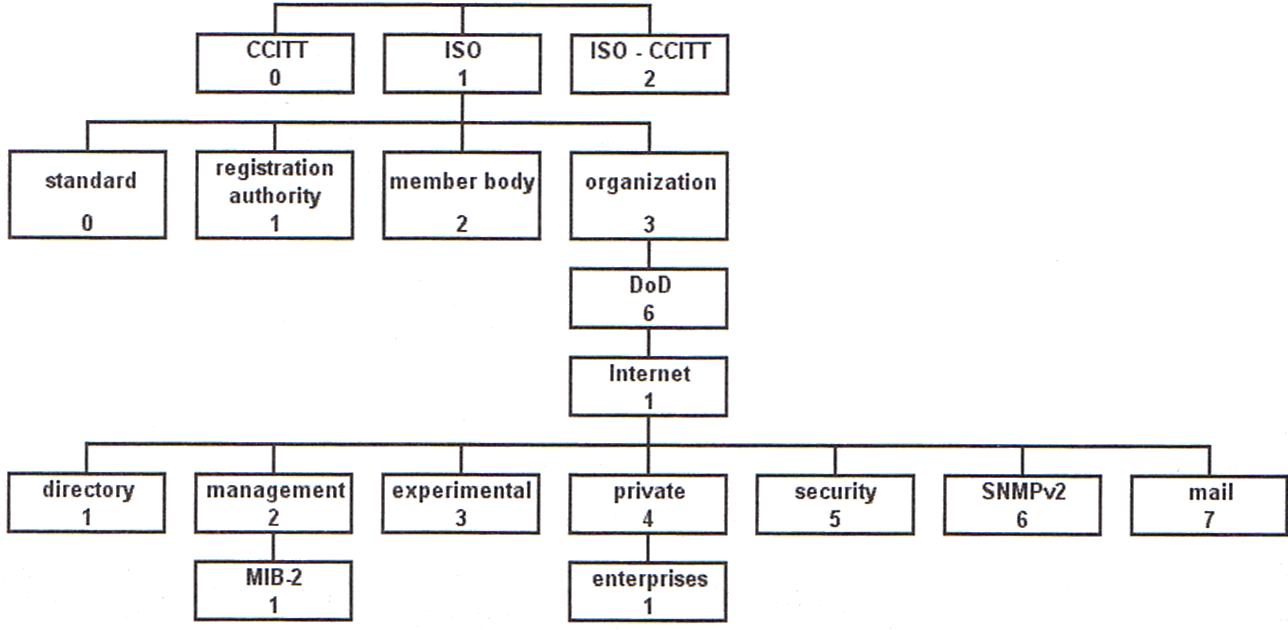
\includegraphics[width=0.95\textwidth]{bilder/mib.png}}
		\caption[Struktur der Management Information Base (MIB)]{Struktur der Management Information Base (MIB)\protect\footnotemark}
		\label{munin-mib}
\end{figure}
\footnotetext{Quelle: \cite{Mu08} S. 156}
Dadurch können die SNMP-Plugins den gewünschten Wert über das Netzwerk abfragen, ohne, dass ein lokal auf dem Munin-Node installiertes Programm notwendig ist.

\newpage

Einen beispielhaften Zugriff auf SNMP-fähige Geräte wird in Abbildung \ref{munin-snmp} gezeigt.

\begin{figure}[ht]
	\centering
	   \fbox{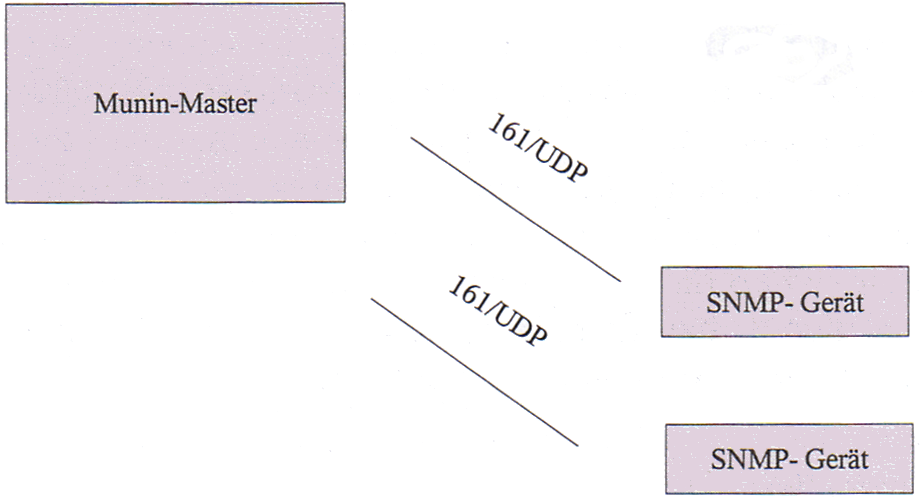
\includegraphics[width=0.85\textwidth]{bilder/snmp.png}}
		\caption[Beispielhafter Zugriff auf SNMP-fähige Geräte]{Beispielhafter Zugriff auf SNMP-fähige Geräte\protect\footnotemark}
		\label{munin-snmp}
\end{figure}
\footnotetext{Quelle: \cite{Mu08} S. 156}

Munin verwendet für SNMP-Plugins eine besondere Namenskonvention.
Alle Plugins dieser Art besitzen den Präfix \textit{snmp\_} auf den die IP-Adresse des SNMP-fähigen Gerätes folgt.
Im folgenden Beispiel wird die Plattenbelegung eines entfernten Knotens überwacht.

\begin{figure}[ht]
	\centering
	   \fbox{
\includegraphics[width=0.85\textwidth]{bilder/snmp-simple.png}}
		\caption{Beispielhafte Verlinkung eines SNMP-Plugins}
		\label{snmp-simple}
\end{figure}

Auch bei diesen SNMP-Plugins gibt es Wildcard-Plugins.
Dabei wird als Suffix im unteren Beispiel der zweite Netzwerkport eines SNMP-fähigen Switches nach Paketfehler abgefragt.

\begin{figure}[ht]
	\centering
	   \fbox{
\includegraphics[width=0.85\textwidth]{bilder/snmp-complex.png}}
		\caption{Beispielhafte Verlinkung eines Wildcard-SNMP-Plugins}
		\label{snmp-complex}
\end{figure}

\newpage

Munin liefert unter anderem folgende SNMP-Plugins mit:

\begin{itemize}
\item \textit{snmp\_\_df} überwacht die Plattenbelegung.
\item \textit{snmp\_\_if\_} ermittelt den Netzwerkdurchsatz.
\item \textit{snmp\_\_if\_err\_} zählt die Paketfehler im Netzwerk.
\item \textit{snmp\_\_sensors\_\_fan} ermittelt die Lüfterdrehzahl.
\item \textit{snmp\_\_load} überwacht die Systemlast.
\item \textit{snmp\_\_processes} ermittelt die Anzahl der laufenden Prozesse.
\item \textit{snmp\_\_users} ermittelt die Anzahl der eingeloggten Benutzer.
\end{itemize}













 \newpage
%\section{Architektur}

Munin verwendet eine sogenannte Master-Node-Architektur, siehe Abbildung \ref{master-munin}.
Hierbei emittelt jeder Rechner seine Messwerte selbst und der Master holt sich diese Daten mittels diverser Agenten, den sogenannten Munin-Nodes, ab.
Deshalb wird der Master lediglich zur Verarbeitung der Überwachungsdaten genutzt.

\begin{figure}[ht]
	\centering
	   \fbox{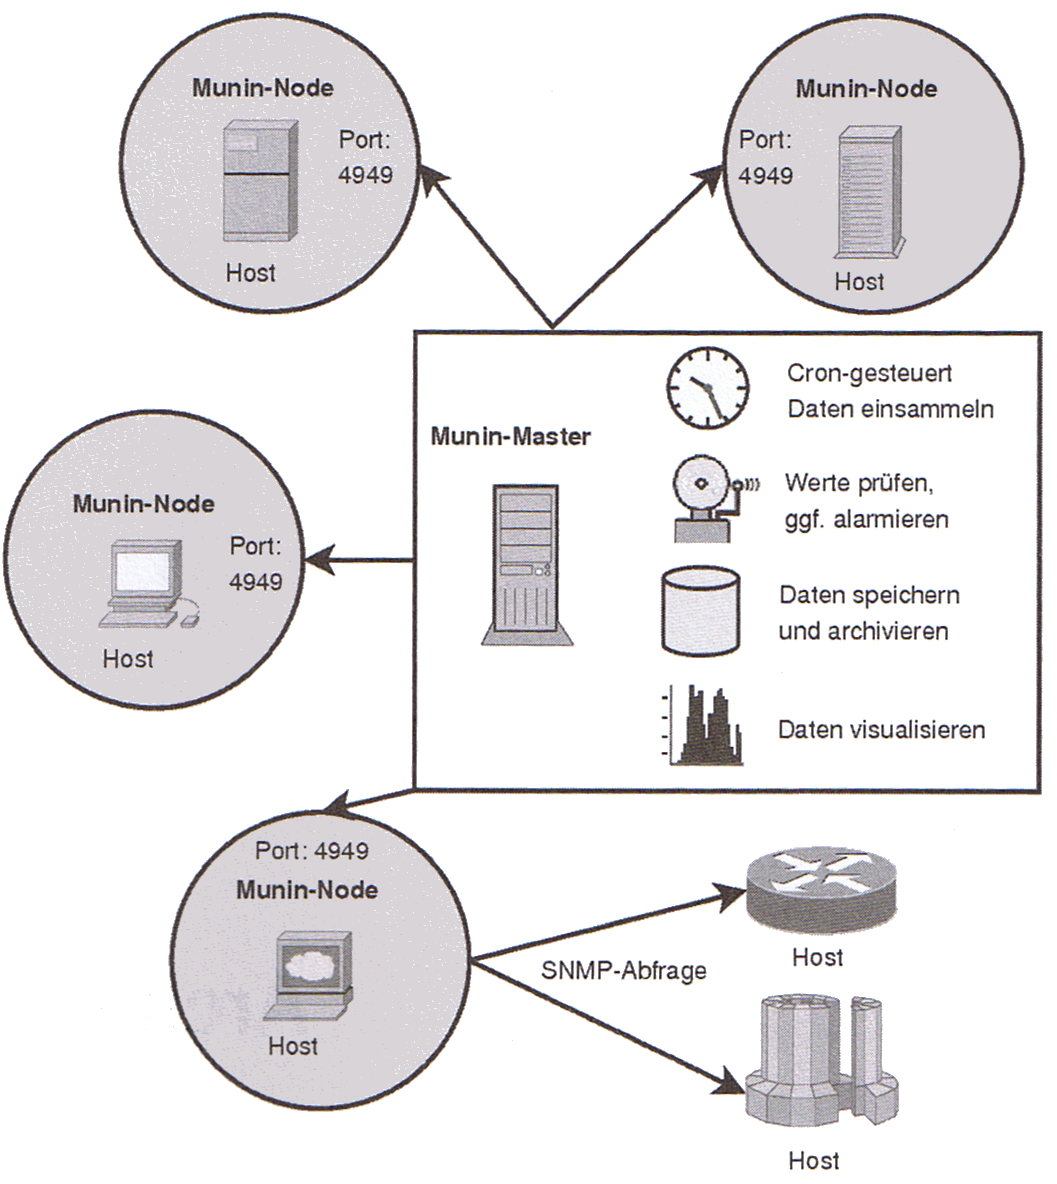
\includegraphics[width=0.85\textwidth]{bilder/master.png}}
		\caption[Munin Master-Node-Konzept]{Munin Master-Node-Konzept\protect\footnotemark}
		\label{master-munin}
\end{figure}
\footnotetext{Quelle: \cite{Mu08} S. 20}

Der Munin-Master ist kein Daemon, sondern besteht aus Skripten, die in regelmäßigen Zeitabstanden als Cron-Job ablaufen:
\begin{itemize}
\item \pictext{munin-update} dient zum Abrufen der Messwerte bei den zu überwachenden Munin-Nodes. Hierbei wird auch die Datenbank aktualisiert oder ggf. erzeugt.
\item \pictext{munin-limits} vergleicht die Messwerte mit ggf. vorgegebenen Schwellwerten und versendet bei Bedarf Benachrichtigungen, wenn Werte das Warnlevel überschreiten, in kritische Bereich gelangen oder wenn Entwarnung gegeben werden kann.
\item \pictext{munin-graph} erzeugt die Munin-Graphen.
\item \pictext{munin-html} dient zum Erstellen der HTML-Seiten der Munin-Übersicht.
\end{itemize}

Standardmäßig werden diese Skripte im fünf Minuten Rythmus aufgerufen.
Dabei baut der Munin-Master viele parallele - im Ausgangszustand unverschlüsselte - TCP-Verbindungen zu den diversen Node-Hosts auf.

Zusätzlich wird für den Betrieb des Munin-Masters auf einem Rechner folgende vorab konfigurierte Software vorausgesetzt:

\begin{itemize}
\item einen Webserver, der Zugang zu den Graphen verschafft.
\item ein Programm mit dem sich die Warnmeldungen versenden lassen. Beispielsweise einen SMTP-Server oder einen Nagios Service Check Acceptor (NSCA), der dafür sorgt, dass der Nagios-Server Alarm schlägt.
\item Werkzeuge und Bibliotheken des \textit{RRDtool}-Projekts\footnote{http://oss.oetiker.ch/rrdtool/} zur Speicherung der Daten und zum Zeichnen der Munin-Graphen.
\end{itemize}


\subsection{Einsammeln der Daten}
Das periodisch ausgeführte Perlskript \pictext{munin-update} kümmert sich um das Abholen neuer Messwerte von den Nodes.
Dazu wird als Erstes die Datei \pictext{munin.conf} geparst, um die zu überwachenden Nodes zu ermitteln.

Ein Eintrag für einen Node-Host in dieser Datei sieht folgendermaßen aus:


\begin{lstlisting}[captionpos=b, caption=Beispielhafte Definition eines Munin-Nodes, label=nodedef, breaklines = true, language=bash]
[munin.example.net]
	address 			localhost
	port				6088
	df.warning			20
	df.critical			10
	contacts			paul
	ping_unilabad.contacts		lang
\end{lstlisting}

Der String in den eckigen Klammern wird als Identifikationsnamen für den Host verwendet und dieser Node wird auch im Webinterface unter diesem Namen aufgelistet.

Das Attribut \textit{address} gibt die IP-Adresse des zu überwachenden Hosts an und mit \textit{port} kann ein vom Standardport (4949) abweichender Port angegeben werden.

Die einzelnen Schwellwerte der verschiedenen Plugins werden auch in diesem Eintrag angegeben, wenn sie von den vorkonfigurierten Werten abweichen sollen.
Dafür wird der Name des Plugins mit den Suffixen \textit{.warning} und \textit{.critical} für die jeweiligen Schwellwerte gesetzt.
Im obigen Beispiel wird \pictext{df} für den freien Festplattenspeicherplatz mit dem Schwellwert von 20\% für Warnungen und 10\% als kritischen Wert für den Host definiert.

Unter dem Attribut \textit{contacts} werden die Kontaktnamen angegeben, die bei einer Überschreitung eines Schwellwerteres kontaktiert werden sollen.
Hierbei gibt es zu sagen, dass diese Überschreitung bei egal welchem Plugin für die Benachrichtigung dieser Kontakte führt.

Soll ein Kontakt nur bei einem bestimmten Plugin benachrichtigt werden, muss es analog zu der Schwellwertdefinition mit dem Pluginnamen und dem Suffix \textit{.contacts} explizit angegeben werden. Hier wird der Kontakt \textit{lang} nur bei einer Überschreitung des Plugins \textit{ping\_unilabad} benachrichtigt.
Bei diesem Plugin wird der Host \textit{unilabad} mit einem Ping überwacht.
Für weitere Details zu dieser Art von Plugin siehe Kapitel \ref{wildcard}.

Weiterhin lässt sich einstellen, dass ein Kontakt generell nur bei kritischen Werten benachrichtigt werden soll.
Die Kontakte müssen zuvor in der \\ \pictext{munin.conf} definiert werden.

Nach der Ermittlung der Nodes werden die Hosts in der Regel parallel nach den neuen Messwerten abgefragt.
Hierfür erzeugt Munin  für jeden in der Konfigurationsdatei angegebenen Rechnern einen eigenen Prozess.
Das parallele Abarbeiten hat den Vorteil, dass die Abfrage nicht bis zum Timeout hängen bleibt, wenn ein einzelner Munin-Node nicht erreichbar ist.
Jedoch verschlingt das Erzeugen eines eigenen Prozesses für jeden Node bei vielen zu überwachenden Rechnern viele Ressourcen, so dass bei größeren Umgebungen viel Arbeitsspeicher und schnelle Multicoreprozessoren unabdingbar sind.

Ein beispielhafte Ausführung eines Munin-Plugins für die Plattenbelegung gibt folgende Werte zurück:

\begin{figure}[ht]
	\centering
	   \fbox{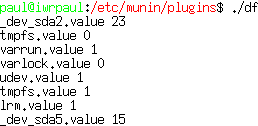
\includegraphics[width=0.6\textwidth]{bilder/df-munin.png}}
		\caption{Beispielhafte Ausführung eines Munin-Plugins}
		\label{df-munin}
\end{figure}
\newpage
Wenn man diese Werte mit den realen Werten vergleicht, erkennt man, dass das Munin-Plugin einfach die Prozentwerte des verbrauchten Speicherplatzes als Wert verwendet.

\begin{figure}[ht]
	\centering
	   \fbox{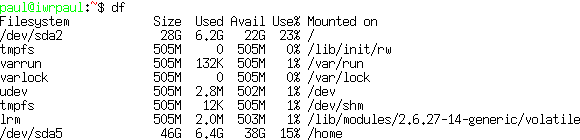
\includegraphics[width=0.85\textwidth]{bilder/df.png}}
		\caption{Reale Werte des Systemtools \textit{df}}
		\label{df}
\end{figure}

Aus diesen Werten erstellt \pictext{munin-graph} automatisch folgenden Graphen:

\begin{figure}[ht]
	\centering
	   \fbox{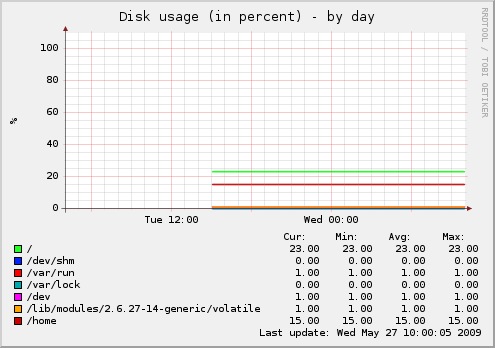
\includegraphics[width=0.85\textwidth]{bilder/df-graph.png}}
		\caption{Visualisierung der Werte des Munin-Plugins \textit{df}}
		\label{df-graph}
\end{figure}

Die über das Netzwerk ermittelten Werte landen nach entsprechender Bearbeitung in RRD-Dateien. 
Im Skript \pictext{munin-update} ist fest eingetragen, welche zeitliche Auflösung die Datenbasis und dadurch auch die Munin-Graphen aufweisen.

Das bedeutet, dass für einen Messpunkt in der Wochenübersicht 30 Minuten - also sechs Messwerte - benötigt werden und für die Monatübersicht werden bereits 48 Messpunkte bzw. zwei Stunden benötigt. Siehe hierfür Tabelle \ref{timeres-tab}.

\begin{table}[!htbp]
\centering
%\begin{twoparttable}
\begin{tabular}{l l}
%\hline
\textbf{Alter der Daten } \hspace{10 mm} & \textbf{Auflösung} \hspace{10 mm} \\
\hline
%\textit{features} & complete\tnote{1} & complete\tnote{1} \\
%\hline
bis zu 30 Stunden & 5 Minuten  \\
\hline
bis zu 9 Tagen & 30 Minuten \\
\hline
bis zu 45 Tagen & 2 Stunden \\
\hline
bis zu 450 Tagen & 1 Tag \\
%\hline
\bottomrule
\end{tabular}
\caption[Zeitliche Auflösung der Datenbasis]{Zeitliche Auflösung der Datenbasis\protect\footnotemark}
\label{timeres-tab}
%\end{twoparttable}
\end{table}
\footnotetext{Quelle: \cite{Mu08} S. 24}


In der Abbildung \ref{4times} konnte der \pictext{munin-node} noch keinen kompletten Tag Messwerte sammeln, weshalb die Jahresübersicht noch keine Messwerte liefern kann und nur mit dem Platzhalterwert \textit{nan} (für nicht defniert) aufgefüllt ist.

\begin{figure}[ht]
	\centering
	   \fbox{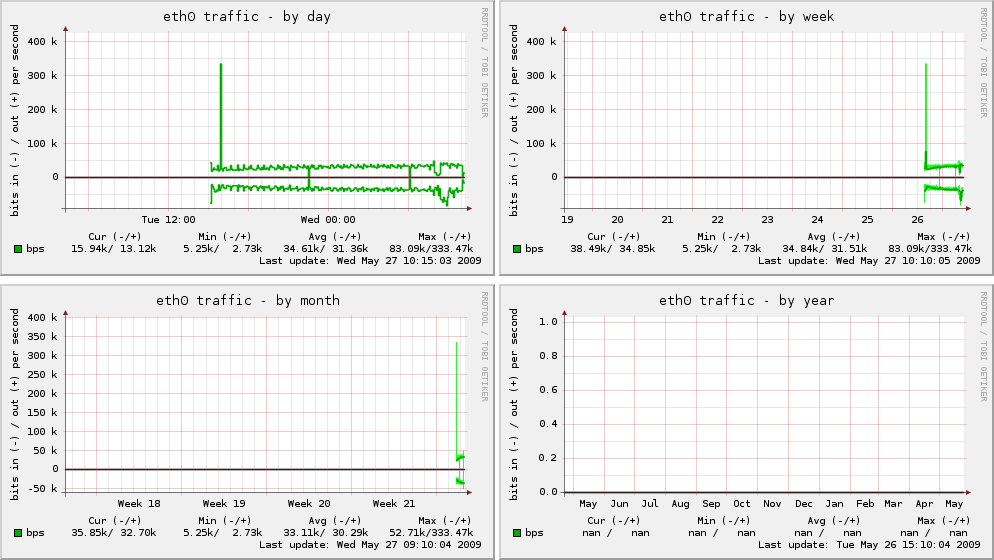
\includegraphics[width=0.9\textwidth]{bilder/4times.png}}
		\caption{Visualisierung der Messwerte in verschiedenen Zeitauflösungen}
		\label{4times}
\end{figure}



\subsection{Round-Robin-Datenbanken}
Round-Robin-Datenbanken sind nicht mit bekannten Datenbanksystemen vergleichbar, da sie in einem proprietären, binären Dateiformat vorliegen.
Daher scheidet der Zugriff per SQL, Texteditor oder über einen Netzwerkport aus.
Um auf Round-Robin-Datenbanken zuzugreifen müssen die dafür entwickelten RRD-Tools verwendet werden.
Diese nehmen die aktuellen Messwerte entgegen und schreiben für jeden Messinterval einen Wert in eine Binärdatei.
Aus dem gesammeltem Datenbestand können dann die Werte visualisiert oder Statistiken erzeugt werden.
Dieser Datenbestand besteht aus sogenannten Round-Robin-Archives.
Dabei handelt es sich um Ableitungen aus den Primärdateien, die mit Hilfe statistischer Auswertungen ermittelt und für die festgelegten Zeitintervalle komprimiert werden.
Die gesamte Anzahl der gespeicherten Datenwerte steht bereits bei der Erzeugung der RRD fest.
Da auch zu Beginn alle Werte mit Platzhaltern aufgefüllt werden, bleibt die Größe einer RRD über die Zeit gleich, siehe Abbildung \ref{rrd-munin}.

\begin{figure}[ht]
	\centering
	   \fbox{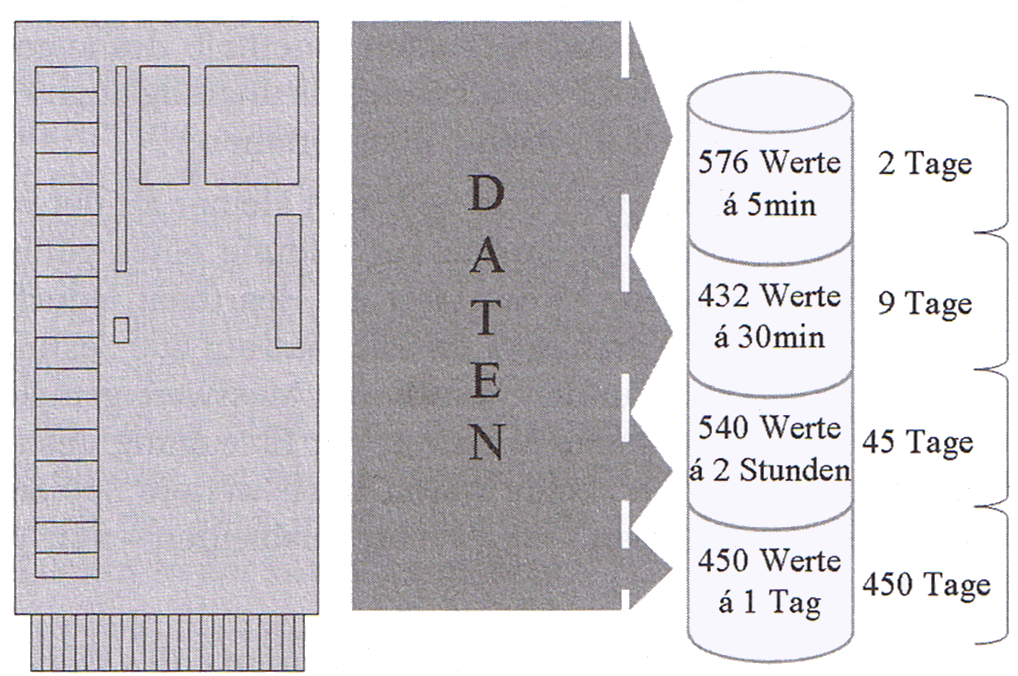
\includegraphics[width=0.76\textwidth]{bilder/rrd.png}}
		\caption[Modell der Round-Robin-Datenbanken]{Modell der Round-Robin-Datenbanken\protect\footnotemark}
		\label{rrd-munin}
\end{figure}
\footnotetext{Quelle: \cite{Mu08} S. 38}

Munin verwendet dieses RRAs als hochauflösende Archive, die die Messwerte des aktuellen Tages, eine etwas komprimierte Fassung zur Darstellung der Daten der laufenden Woche sowie - noch stärker komprimiert - die Daten für den aktuellen Monat und das Jahr enthalten.
%Siehe hierfür Abbildung [?].
Die Komprimierung wird so realisiert, dass Mittelwerte aus der feineren Zeitauflösung errechnet werden und zusätzlich noch spezielle Archivierungsregeln beim Erstellen der RRD-Datei berücksichtigt werden.

Aus diesen Datensätzen mit unterschiedlichen Zeitauflösungen erstellt Munin automatisch Graphen über die entsprechenden Zeiträume, siehe Abbildung \ref{all4}.

\begin{figure}[ht]
	\centering
	   \fbox{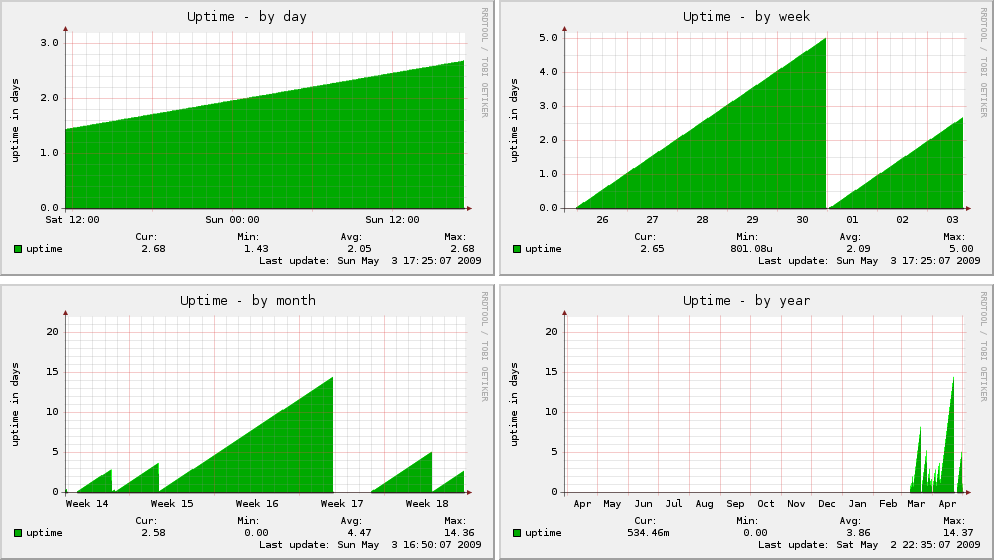
\includegraphics[width=0.95\textwidth]{bilder/all4.png}}
		\caption{Übersicht der \textit{Uptime}}
		\label{all4}
\end{figure}

\newpage

\subsection{Einbindung und Konfiguration der Plugins}
\label{plugins}
Munin bringt bereits eine Sammlung von Plugins bei der Installation mit.
Diese befinden sich in einem Bibliotheksverzeichnis.
Wenn diese Plugins verwendet werden sollen um einen Node zu überwachen, müssen sie in einem Service-Verzeichnis verlinkt sein, damit der Daemon \pictext{munin-node} darauf zugreifen kann.
Dieser Daemon muss sich auf dem zu überwachenden Host befinden und dient als "`Agent"' für den Munin-Master, da der Daemon auf seinem Port nach Aufforderungen durch den Master horcht.
Ein solcher Daemon ist für Linux und für Windows verfügbar, wobei der für Windows weniger Funktionen bietet.
Die einzelnen Tests laufen auf den Nodes unabhängig von der Abfrage des Masters.
Wenn der Master die aktuellen Daten nicht abholt, wird dieser Datenbestand durch die neuen Informationen ausgetauscht und werden bei der nächsten Anfrage an den Master gesendet.

Auf den Graphen im Webinterface wird dieser Zeitraum als Lücke dargestellt, siehe Abbildung \ref{gap}.

\begin{figure}[ht]
	\centering
	   \fbox{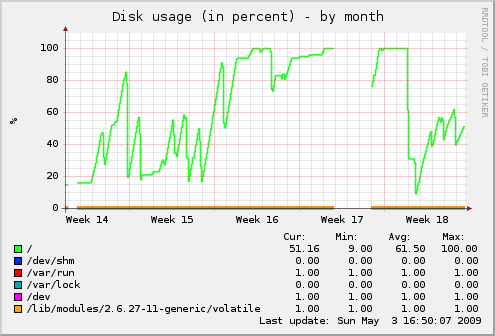
\includegraphics[width=0.852\textwidth]{bilder/gap.png}}
		\caption{Fehlende Messwerte werden als Lücke dargestellt}
		\label{gap}
\end{figure}

Der \pictext{munin-node}-Daemon kannn so konfiguriert werden, dass er nur auf Anfragen von einer bestimmten IP reagiert, einen anderen Port verwendet oder nur auf einer bestimmten IP lauscht.

Damit der Daemon weiss, welche Daten er liefern muss, wird das zuvor erwähnte Service-Verzeichnis verwendet.
Hier werden Verlinkungen zu den eigentlichen Plugins gespeichert.
Eine beispielhafte Verlinkung wird in Abbildung \ref{lns} gezeigt.

\begin{figure}[ht]
	\centering
	   \fbox{
\includegraphics[width=0.85\textwidth]{bilder/lns.png}}
		\caption{Beispielhafte Verlinkung eines Munin-Plugins}
		\label{lns}
\end{figure}

\subsubsection{Wildcard-Plugins}
\label{wildcard}
Falls der Name des Plugins mit einem Unterstrich endet, handelt es sich um ein sogenanntes \textit{Wildcard}-Plugin.
Solche Plugins erwarten in der Bezeichnung des Links spezifische Parameter für die Ausführung der Tests.

Beispielsweise verwendet das zuvor verwendete Plugin \textit{ping\_} als Parameter den Namen oder die IP-Adresse des anzupingenden Hosts.
Die Verlinkung aus dem Bibliotheksverzeichnis in das Service-Verzeichnis würde dann folgendermaßen ausschauen:
\begin{figure}[ht]
	\centering
	   \fbox{
\includegraphics[width=0.85\textwidth]{bilder/lnw.png}}
		\caption{Beispielhafte Verlinkung eines Wildcard-Plugins}
		\label{lnw}
\end{figure}

Hier wird der Host \textit{localhost} angepingt und diese Daten auf dem Master gespeichert und später in einem Graphen visualisiert.

\newpage

\subsubsection{SNMP-Plugins}
Es ist auch möglich Informationen über den zu überwachenden Host in Erfahrung zu bringen, ohne, dass ein \pictext{munin-node}-Daemon auf dem Host installiert ist.
Dies wird durch das Simple Network Management Protocol (SNMP) realisiert.
Durch SNMP kann auf die strukturierte Datenhaltung der MIB in den entfernten Netzwerkknoten zugegriffen werden.
\begin{quote}"`Die Management Information Base (MIB) dient als SNMP-Informations-struktur und besteht aus einem hierarchischen, aus Zahlen aufgebauten Namensraum. Ähnliche Struktur wie andere hierarchische Verzeichnisdiensten wie DNS oder LDAP."'\end{quote}
\begin{flushright}
Quelle: \cite{Barth08} S.233
\end{flushright}

Die MIB-Struktur ist folgendermaßen aufgebaut:

\begin{figure}[ht]
	\centering
	   \fbox{\includegraphics[width=0.95\textwidth]{bilder/mib.png}}
		\caption[Struktur der Management Information Base (MIB)]{Struktur der Management Information Base (MIB)\protect\footnotemark}
		\label{munin-mib}
\end{figure}
\footnotetext{Quelle: \cite{Mu08} S. 156}
Dadurch können die SNMP-Plugins den gewünschten Wert über das Netzwerk abfragen, ohne, dass ein lokal auf dem Munin-Node installiertes Programm notwendig ist.

\newpage

Einen beispielhaften Zugriff auf SNMP-fähige Geräte wird in Abbildung \ref{munin-snmp} gezeigt.

\begin{figure}[ht]
	\centering
	   \fbox{\includegraphics[width=0.85\textwidth]{bilder/snmp.png}}
		\caption[Beispielhafter Zugriff auf SNMP-fähige Geräte]{Beispielhafter Zugriff auf SNMP-fähige Geräte\protect\footnotemark}
		\label{munin-snmp}
\end{figure}
\footnotetext{Quelle: \cite{Mu08} S. 156}

Munin verwendet für SNMP-Plugins eine besondere Namenskonvention.
Alle Plugins dieser Art besitzen den Präfix \textit{snmp\_} auf den die IP-Adresse des SNMP-fähigen Gerätes folgt.
Im folgenden Beispiel wird die Plattenbelegung eines entfernten Knotens überwacht.

\begin{figure}[ht]
	\centering
	   \fbox{\includegraphics[width=0.85\textwidth]{bilder/snmp-simple.png}}
		\caption{Beispielhafte Verlinkung eines SNMP-Plugins}
		\label{snmp-simple}
\end{figure}

Auch bei diesen SNMP-Plugins gibt es Wildcard-Plugins.
Dabei wird als Suffix im unteren Beispiel der zweite Netzwerkport eines SNMP-fähigen Switches nach Paketfehler abgefragt.

\begin{figure}[ht]
	\centering
	   \fbox{\includegraphics[width=0.85\textwidth]{bilder/snmp-complex.png}}
		\caption{Beispielhafte Verlinkung eines Wildcard-SNMP-Plugins}
		\label{snmp-complex}
\end{figure}

\newpage

Munin liefert unter anderem folgende SNMP-Plugins mit:

\begin{itemize}
\item \textit{snmp\_\_df} überwacht die Plattenbelegung.
\item \textit{snmp\_\_if\_} ermittelt den Netzwerkdurchsatz.
\item \textit{snmp\_\_if\_err\_} zählt die Paketfehler im Netzwerk.
\item \textit{snmp\_\_sensors\_\_fan} ermittelt die Lüfterdrehzahl.
\item \textit{snmp\_\_load} überwacht die Systemlast.
\item \textit{snmp\_\_processes} ermittelt die Anzahl der laufenden Prozesse.
\item \textit{snmp\_\_users} ermittelt die Anzahl der eingeloggten Benutzer.
\end{itemize}













 \newpage



\section{Abbildungsverzeichnis}
\listoffigures
\newpage
\section{Tabellenverzeichnis}
\listoftables
\newpage
\renewcommand{\lstlistlistingname}{}
\section{Codelistingverzeichnis}
\lstlistoflistings
\newpage
\renewcommand{\refname}{} 
\section{Literaturverzeichnis}
\begin{thebibliography}{xxxxxx}
	 \bibitem[Pro02]{Pro02}Ernst Probst (2002) "`Nordische Göttersagen"', \newline ISBN13: 978-3-936326-05-5, Einsichtnahme: 02.05.2009\\
	 
	 \bibitem[Munin08]{Mu08} Gabriele Pohl und Michael Renner (2008) 
	 "`Munin - Graphisches Netzwerk- und System-Monitoring"', \newline ISBN13: 978-3-937514-48-2, Einsichtnahme: 05.04.2009\\
	 
	 \bibitem[Barth08]{Barth08}Wolfgang Barth (2008) "`Nagios - System- und Netzwerk-Monitoring"' 2. Auflage, \newline ISBN13: 978-3-937514-46-8, Einsichtnahme: 14.05.2009\\
	 
\end{thebibliography}
\newpage
\section{Anhang}


\end{document}



